\documentclass[lang=cn,10pt]{elegantbook}

\title{实变函数}
\subtitle{东邪的第一本书}

\author{Dx}

\date{25/5/2025}

\bioinfo{自定义}{信息}

\extrainfo{不要以为抹消过去,重新来过,即可发生什么改变。—— 比企谷八幡}

\setcounter{tocdepth}{3}

\logo{logo-blue.png}
\cover{cover.jpg}

% 本文档命令
\usepackage{array}
\newcommand{\ccr}[1]{\makecell{{\color{#1}\rule{1cm}{1cm}}}}

% 修改标题页的橙色带
% \definecolor{customcolor}{RGB}{32,178,170}
% \colorlet{coverlinecolor}{customcolor}
\let\oldliminf\liminf
\renewcommand{\liminf}{\mathop{\oldliminf}\limits}

\let\oldlimsup\limsup
\renewcommand{\limsup}{\mathop{\oldlimsup}\limits}
\begin{document}

\maketitle
\frontmatter

\tableofcontents

\mainmatter

\chapter{第一章 基础知识}
实变函数这门课程让我学会了另一种积分的方式,对集合的理解越发深刻。



  
\section{集合}

主要学习集

\subsection{集合列的极限}
集合列就像函数列是一列集和,初次看到这种交并符号写在一起,本能会头疼下面我来讲述一下如何克服这件事。首先把最讨厌的$\infty$给去掉,举一个特例再理解会容易的多。
\begin{definition}
    设 $\{A_n\}_{n=1}^\infty$ 是 $\mathbb{R}^n$ 中的一列集合,则:

\begin{align*}
\liminf_{n \to \infty} A_n &= \bigcup_{k=1}^\infty \bigcap_{n = k}^\infty A_n \\[1em]
\limsup_{n \to \infty} A_n &= \bigcap_{k=1}^\infty \bigcup_{n = k}^\infty A_n
\end{align*}

若 $\liminf_{n \to \infty} A_n = \limsup_{n \to \infty} A_n$,则称集合列 $\{A_n\}$ 极限存在,记为:

\[
\lim_{n \to \infty} A_n = \liminf_{n \to \infty} A_n = \limsup_{n \to \infty} A_n
\]
\end{definition}
比如说我们先看第一个函数列下极限,我们就取 $n=3$ 看看会发生什么。

$k=1$ 开始,$A_1 \bigcap A_2 \bigcap A_3 = B_1$,此时从 $k=1$ 开始我们生成了第一项 $B_1$,$B_1$ 中的元素是 $A_1,A_2,A_3$ 中都有的。

然后我们让 $k=2$,$A_2 \bigcap A_3 = B_2$,$B_2$ 中是 $A_2,A_3$ 里面都有的元素,那么我们可以知道 $B_2$ 中的元素是比 $B_1$ 多的。

然后 $k=3$,$B_3 = A_3$,此时我们将 $B_1,B_2,B_3$ 并起来,里面的元素就是:$A_1,A_2,A_3$ 都有的、$A_2,A_3$ 都有的、$A_3$ 有的。可以有 $A_3$ 有但 $A_1,A_2$ 没有的元素。
$B_1$ 里面的是所有 $A_n$ 里面都有的元素,$B_2$ 里面的是所有 $A_n$ 除了第一项都有的元素,$B_m$ 是除了前 $m$ 项后面都有的元素。
如果我们将 $3$ 推广到 $n$,那就是 $B_1$ 到 $B_n$ 的并,任意一个在这个并里面的元素x,只要出现在了$B_m$里那么他一定会出现在除了前$m$项,后面所有的项。
\[
\forall x \in \liminf_{n \to \infty} A_n, \quad \exists N \in \mathbb{N}, \; \forall m > N, \; x \in A_m
\] 
这个和我们基础的数列极限的样子很像了,函数列上极限同理:$B_1$ 就是所有项的并,$B_2$ 就是除了第一项所有项的并,$B_3$ 就是除了前两项,所有项的并。

\par

记住每交一次都是一次筛选和剔除。第一次$B_1和B_2$的交就把 $A_1$ 独有的元素剔除了因为$B_2$中没有$A_1$但如果A1有的元素,后面Am也有。这样的元素还是会在B2,当然也在B1中也就在B1交B2里面,第二次交(即 $B_1, B_2, B_3$ 的交)在剔除 $A_1$ 独有元素的基础上,又剔除了 $A_2$ 独有的元素。

\par

依此类推到无穷,剩下的元素就是无限次出现在 $A_n$ 中的元素。注意:不是每个 $A_n$ 都有的元素。

例如:设 $A_{2n+1} = \{1\}$,$A_{2n} = \{2\}$,那么这个集合列的上极限是 $\{1, 2\}$。
\subsection{开集与闭集}
这将讲述开集闭集这两个实分析重要的集合也是一个非常重要的基础知识。有一个先入为主的印象就是一个集合是一坨点是在一起的,然而并不是集合可以是离散的就是东一个点西一个点彼此离的很远。
集合是由一些点组成的所以具有什么种类的点决定了这个集合是什么样的。集合中的点有以下类型内点,聚点,孤立点,边界点
\begin{definition}
    \textbf{内点}:若$\exists r>0$,使得开球 $B(x, r) \subset E$,则称点 $x$ 是 $E$ 的内点。\\
    \textbf{聚点}:设 $E \subset \mathbb{R}^n$,若对任意 $\varepsilon > 0$,开球 $B(x, \varepsilon)$ 中除 $x$ 本身外含有 $E$ 中的点,即
\[
(B(x, \varepsilon) \setminus \{x\}) \cap E \neq \varnothing,
\]
则称点 $x$ 是 $E$ 的聚点。\\
\textbf{边界点}:设 $E \subset \mathbb{R}^n$,若对任意 $\varepsilon > 0$,开球 $B(x, \varepsilon)$ 与 $E$ 和 $E^c$ 都有交集,即
\[
B(x, \varepsilon) \cap E \neq \varnothing,\quad B(x, \varepsilon) \cap E^c \neq \varnothing,
\]
则称点 $x$ 是 $E$ 的边界点。\\
\textbf{孤立点}:设 $E \subset \mathbb{R}^n$,若 $x \in E$,且存在 $\varepsilon > 0$ 使得
\[
B(x, \varepsilon) \cap E = \{x\},
\]
则称 $x$ 是 $E$ 的孤立点。
\end{definition}
设有一个集合叫做E,E中所有内点的集合叫内域$\mathring{E}$,E中所有的聚点的集合叫导集E',
\begin{remark}
    开球是什么呢?开区间大家都知道比如(0,1),注意开区间都是这点是在一块的是不离散的,所以开区间是开集但是开集不一定是开区间,那么开球就是把开区间拓展到维度,比如一位的是后半径r作用范围就是数轴开球就是开区间,二维的时候到平面上了开球就是以x为圆心,r为半径内所有的点。\\内点要求存在r>0,当点都在以内点为圆心r为半径的圆内的点都在E里面。也就是他周边的点都必须是E中的点。\\聚点是要求身边一直有E中的点,重点是要求除了自己本身还有其他属于E的点,内点都是聚点因为内点总有围着一他一圈的点都是属于E的,但是聚点不一定是内点因为聚点要求的是有E中的点,而不是全都是E中的点。\\ps看见任意就像构造这个数学直觉先记住以后有的是要用的时候。\\E中不是聚点就是孤立点,边界点要求开球B(x,r)中既有属于E的点也有不属于E的点但是他没有强调这个点不能是x本身所以边界点不一定是聚点。\\给举一个例子就明白了比如一个集合里面的元素是单位圆中和单位圆上所有的点和(3,0)这个点的并,圆边界上和(3,0)都是边界点,圆去掉边界点剩下的部分就是内点,整个圆中和圆上的点都是聚点,聚点聚点顾名思义聚在一起的点。只有(3,0)这个点孤零零在圆外他就是孤立点。
\end{remark}

\subsection{可数集与不可数集}
我们都学过整数集,实数集等等基础的集合,那么我们如果想知道一个集合到底有多大怎么办呢,我要对集合进行定量。下面引入定义可列集,有限集与不可数集。
\begin{definition}
    与自然数集N对等的集合称为可列集
\end{definition}
什么叫与$\mathbb{N}$与等呢,就是可以和$\mathbb{N}$中元素构成一一映射,可列可列如果你能把一个集合中的元素一个一个列出来也是你判定是不是可列集的一种方式,我先举一个不可数集的例子吧$\mathbb{R}$,如果我们尝试把R中的元素一个一个列出来会发生什么1然后下一个数比1大按照升序排列的话,那是1.0000……1你永远可以往里面加更多的0下一个数你压根找不到也列不出来。\\
有限集顾名思义集合内的元素有限比如说{0,1},元素就两个显然是有限集,有限集和可列集组成可数集,不可数集和可列集都是无限集。
\begin{theorem}
    可数个可列集的并是可列集
\end{theorem}
我们知道一旦涉及到无限很多性质就会被破坏,$\sum_{n=1}^{\infty}\frac{1}{n}$与$
  \sum_{n=1}^{N} \frac{1}{n}$,前者的和是无限的,后者的和是有限的。包括数分中学习的函数列一致收敛就是为了保住就算引入无穷也能保持函数列中每一项的性质比如连续,可微,可导。在集合论的框架下,“可数性”在一定程度上可以看作是保留结构与性质的上限。对于可数个对象的集合,我们仍可以通过排列、穷举、逐项分析等手段加以控制和刻画。但一旦进入不可数集合(如实数集)的范畴,许多原本可控的性质就可能被打破。

\subsection{开集的作用}

\begin{proposition}
    任何一个开集都可以写成可数个开区间的无交并
    开集都能写成开集的并
\end{proposition}
开区间这个基础的结构较好的集合是我们做题的需要平凡构造的,因为如果点都是离散的那么很多很多公式定理都不能用。数学的核心就是拆分问题,将复杂的问题抽丝剥茧一般拆解成简单的问题。就像有时候我们会将无限拆分成有条件的无限和其余有限部分。将开集拆分成开区间,再在每一个开区间上讨论也起到了简化问题的效果。而且开集里面都是内点那么根据内点的定义自动可以构造一个开球B(x,r)属于开集。



\subsection{集合的完备性}
\begin{theorem}
    致密性定理:有界点列都有收敛子列\\
    聚点定理:有界无限点集必有聚点
\end{theorem}
有界是一种限制,当无限的点放在一个有限的空间内他们必定在一个空间内聚集。想想挤地铁,不断有人进来周围原来从没有人变得越来越多人。
\begin{theorem}[闭区间套定理]{}
设有闭区间列 $\{[a_n, b_n]\}$,若:

\begin{enumerate}
  \item $[a_1, b_1] \supset [a_2, b_2] \supset \cdots \supset [a_n, b_n] \supset \cdots$;
  \item $\displaystyle \lim_{n \to \infty} (b_n - a_n) = 0$,
\end{enumerate}

则存在唯一实数 $l$ 属于所有的闭区间
\[
\left( \bigcap_{n=1}^\infty [a_n, b_n] = \{l\} \right),
\]
且有
\[
\lim_{n \to \infty} a_n = \lim_{n \to \infty} b_n = l.
\]
\end{theorem}

闭区间套的作用就是找到你要找到的一个点
\begin{proof}
    条件1 数列${a_n}$单调递增有上界$b_1$,数列${b_n}$单调减少有下界$a_1$就是
    \[
a_1 \leqslant a_2 \leqslant \cdots \leqslant a_n
\leqslant \cdots \leqslant b_n \leqslant \cdots
\leqslant b_2 \leqslant b_1.
\]
单增+有界=收敛 数列{$a_n$}收敛,设$\lim_{n \to \infty} a_n = l$\\
$\lim_{n \to \infty} b_n = \lim_{n \to \infty} (b_n - a_n + a_n) = \lim_{n \to \infty} (b_n - a_n) + \lim_{n \to \infty} a_n = 0 + l = l.$
   \\1表示最后趋近于0的区间被所有区间包含 \\   
 2表示区间长度趋近于0  an数列单增从左往右收缩区间,bn单减从右往左收缩区间。用条件就得从要求的东西身边凑出条件的形式 
 \[
\lim_{n \to \infty} a_n = \lim_{n \to \infty} b_n = l.
\]
那这个闭区间套定理怎么用呢?下面我们会在确界定理里面用到,想要用闭区间套定理定理就得干两件事第一构造嵌套的闭区间,第二保证最小的区间长度趋紧于0,和吃鸡缩小毒圈一样。
\begin{theorem}[确界定理]{}
若非空数集E有上界(下界),则数集E存在唯一的上确界(下确界)
    
\end{theorem}
上确界是一个确定的点,我们就考虑用闭区间套来找到这个点。
要用到闭区间套定理,我们就要按照一定规则构造出嵌套的不区间。我们首先要构造出最大的闭区间也就是$[a_1,b_1]$,a1属于E,E有上界,我们取一个上界b1\\我们这次用的是二分法。我们本次的规则叫P*\\
1)$[a_1,b_1]$的右侧没有数集E的点
2)$[a_1,b_1]$中至少包含有数集E的一个点,将具有性质1,性质2点闭区间叫具有P*的闭区间。
然后我们用二分法把$[a_1,b_1]$分成\\
\begin{tabular}{|c|c|}
  \hline
  $\left[a_1,\dfrac{a_1 + b_1}{2}\right]$ & $\left[\dfrac{a_1 + b_1}{2}, b_1\right]$ \\
  \hline
  定有2 & 定有1 \\
  \hline
  若有1 & 则无2 \\
  \hline
  若无1 & 则有2 \\
  \hline
\end{tabular}
将同时具有性质 1 和性质 2 的区间再次二等分,然后从两个新产生的子区间中选出哪个符合性质 $P^*$,如此不断缩小区间长度,直到逼近上确界 $l$。

事实上,性质 1 的作用是确保上确界 $l$ 位于每一个 $[a_n, b_n]$ 中,而性质 2 则是确保区间 $[a_n, b_n]$ 的左端点 $a_n$ 至少还在集合 $E$ 中。

若 $a_n$ 和 $b_n$ 都不在 $E$ 中,显然就无法找到上确界。\\
\begin{definition}
    cantor三分集,替换二分法。
\end{definition}
\begin{theorem}[有限覆盖定理]\label{thm:HB-interval}
设 $[a,b]$ 为实数轴上的闭区间,$\{U_\alpha\}_{\alpha\in A}$ 为 $[a,b]$ 的一族开覆盖,
即
\[
  [a,b] \subset \bigcup_{\alpha\in A} U_\alpha,\qquad
  U_\alpha \text{ 开}.
\]
则存在有限指标 $\alpha_1,\dots,\alpha_m\in A$,使得
\[
  [a,b] \subset \bigcup_{j=1}^m U_{\alpha_j}.
\]
\end{theorem}
\begin{proof}
设开覆盖族 $\mathcal{S}$ 覆盖闭区间 $[a,b]$.
\medskip

\noindent\textbf{第一步\;构造上确界:}

令
\[
  A=\bigl\{\,x \mid x\in[a,b],\;[a,x]\text{ 可以由 }\mathcal{S}
  \text{ 的有限个开区间覆盖}\,\bigr\}.
\]

由于 $\mathcal{S}$ 是开覆盖,存在开区间 $(\alpha,\beta)\in\mathcal{S}$ 使 $a\in(\alpha,\beta)$,
从而可取 $x>a$ 且 $x\in(\alpha,\beta)$,此时 $[a,x]\subset(\alpha,\beta)$,
显然 $[a,x]$ 被有限个开区间覆盖,故 $A\neq\varnothing$.
又因 $A\subset[a,b]$,故 $A$ 有上界,于是由确界原理可设
\[
  c:=\sup A,\qquad c\le b.
\]

\noindent\textbf{第二步\;证明 $c=b$:}

若设 $c<b$,则由于 $\mathcal{S}$ 覆盖 $[a,b]$,必存在开区间
$(\gamma,\delta)\in\mathcal{S}$ 使 $c\in(\gamma,\delta)$,于是
\[
  \gamma < c < \delta.
\]
由 $c=\sup A$ 可知 $\exists\,x'\in(\gamma,c)$ 使 $x'\in A$,
于是 $[a,x']$ 有有限覆盖;再加上 $(\gamma,\delta)$,
可得 $[a,c]$ 亦有有限覆盖,这与 $c$ 为 $A$ 的上确界矛盾。
因此 $c<b$ 不成立,只能有
\[
  c=b,\qquad\text{即 } \sup A = b.
\]

\noindent\textbf{第三步\;补齐右端点得到有限覆盖:}

因 $b\in[a,b]$,仍可在 $\mathcal{S}$ 中取开区间 $(\xi,\eta)$ 使 $b\in(\xi,\eta)$。
由 $b=\sup A$ 可再取 $x''\in(\xi,b)$ 满足 $x''\in A$。
此时 $[a,x'']$ 已有有限覆盖,再补上 $(\xi,\eta)$,
便得到整个闭区间
\[
  [a,b]=[a,x'']\cup[x'',b]
\]
的有限覆盖,从而覆盖族 $\mathcal{S}$ 存在有限子覆盖。

至此,有限覆盖定理得证。
\end{proof}
有限覆盖定理,证明有限是关键条件是开区间集S覆盖闭区间[a,b],结论是S中存在有限个开区间也覆盖闭区间[a,b]

A是所有x的集合,对x的要求是[a,x]可以被有限覆盖

开区间集S覆盖[a,b]所以集合中存在一个集合(α,β)可以覆盖[a,x]只要[a,x]足够小无论如何是能找到一个比他大的区间把他覆盖掉的。

x的极限就是c。假设[a,c]就是能被有限覆盖的极限了

从S的集合里面找一个区间(γ ,δ)里面有c的,从γ 到c再找一个数x‘

把之前用于覆盖x’到c的若干集合换成(γ ,δ)那么此时能有限覆盖的就是[a,δ],与[a,c]就是可以有限覆盖的极限是矛盾的除非c=b,所以c=b\\
\begin{theorem}[柯西收敛准则]
数列 $\{a_n\}$ 收敛 $\Longleftrightarrow \forall \varepsilon > 0,\; \exists N \in \mathbb{N}_+,\; \forall n, m > N,\; |a_n - a_m| < \varepsilon$.
\end{theorem}

\begin{proof}
\textbf{(必要性 $\Rightarrow$)}  
设 $\{a_n\}$ 收敛于 $a$,即 $\lim\limits_{n\to\infty} a_n = a$。  
则对于任意 $\varepsilon > 0$,存在 $N \in \mathbb{N}_+$,使得当 $n > N$ 时,有
\[
|a_n - a| < \frac{\varepsilon}{2},\quad |a_m - a| < \frac{\varepsilon}{2}.
\]
从而有
\[
|a_n - a_m| \leq |a_n - a| + |a_m - a| < \frac{\varepsilon}{2} + \frac{\varepsilon}{2} = \varepsilon.
\]
因此 $\{a_n\}$ 是柯西列。

\medskip

\textbf{(充分性 $\Leftarrow$)}  
我们首先证明数列 $\{a_n\}$ 有界。

取 $\varepsilon = 1$,根据假设,存在 $N_1 \in \mathbb{N}_+$,使得当 $n > N_1$ 时,对于任意 $m_0 \leq N_1$,都有
\[
|a_n - a_{m_0}| < 1.
\]
从而有
\[
|a_n| \leq |a_n - a_{m_0}| + |a_{m_0}| < 1 + |a_{m_0}|.
\]

取
\[
M = \max\left\{ |a_1|, |a_2|, \dots, |a_{N_1}|, 1 + |a_{m_0}| \right\},
\]
则对任意 $n \in \mathbb{N}_+$,有 $|a_n| \leq M$,即数列 $\{a_n\}$ 有界。

根据致密性定理(定理 5),数列 $\{a_n\}$ 存在一个收敛的子列 $\{a_{n_k}\}$,设其极限为
\[
\lim_{k \to \infty} a_{n_k} = a.
\]

接下来证明 $\lim\limits_{n\to\infty} a_n = a$。

任意给定 $\varepsilon > 0$,根据柯西列性质,存在 $N \in \mathbb{N}_+$,使得当 $n, m > N$ 时,
\[
|a_n - a_m| < \varepsilon.
\]
又由于 $\lim a_{n_k} = a$,所以存在 $k_0$,使得当 $k > k_0$ 时,
\[
|a_{n_k} - a| < \varepsilon.
\]

令 $L = \max\{N, n_{k_0}\}$,则对任意 $n > L$,存在 $k > k_0$,使得
\[
|a_n - a_{n_k}| < \varepsilon,\quad |a_{n_k} - a| < \varepsilon.
\]
从而
\[
|a_n - a| \leq |a_n - a_{n_k}| + |a_{n_k} - a| < \varepsilon + \varepsilon = 2\varepsilon.
\]
因为 $\varepsilon$ 任意,故有 $\lim\limits_{n\to\infty} a_n = a$,即 $\{a_n\}$ 收敛。

\end{proof}
先证明有界无限 然后就可以用致密性构造收敛子列

最后用以知道的条件通过做差说明两个点极限一样

\end{proof}
\chapter{第二章测度}
\section{勒贝格测度}
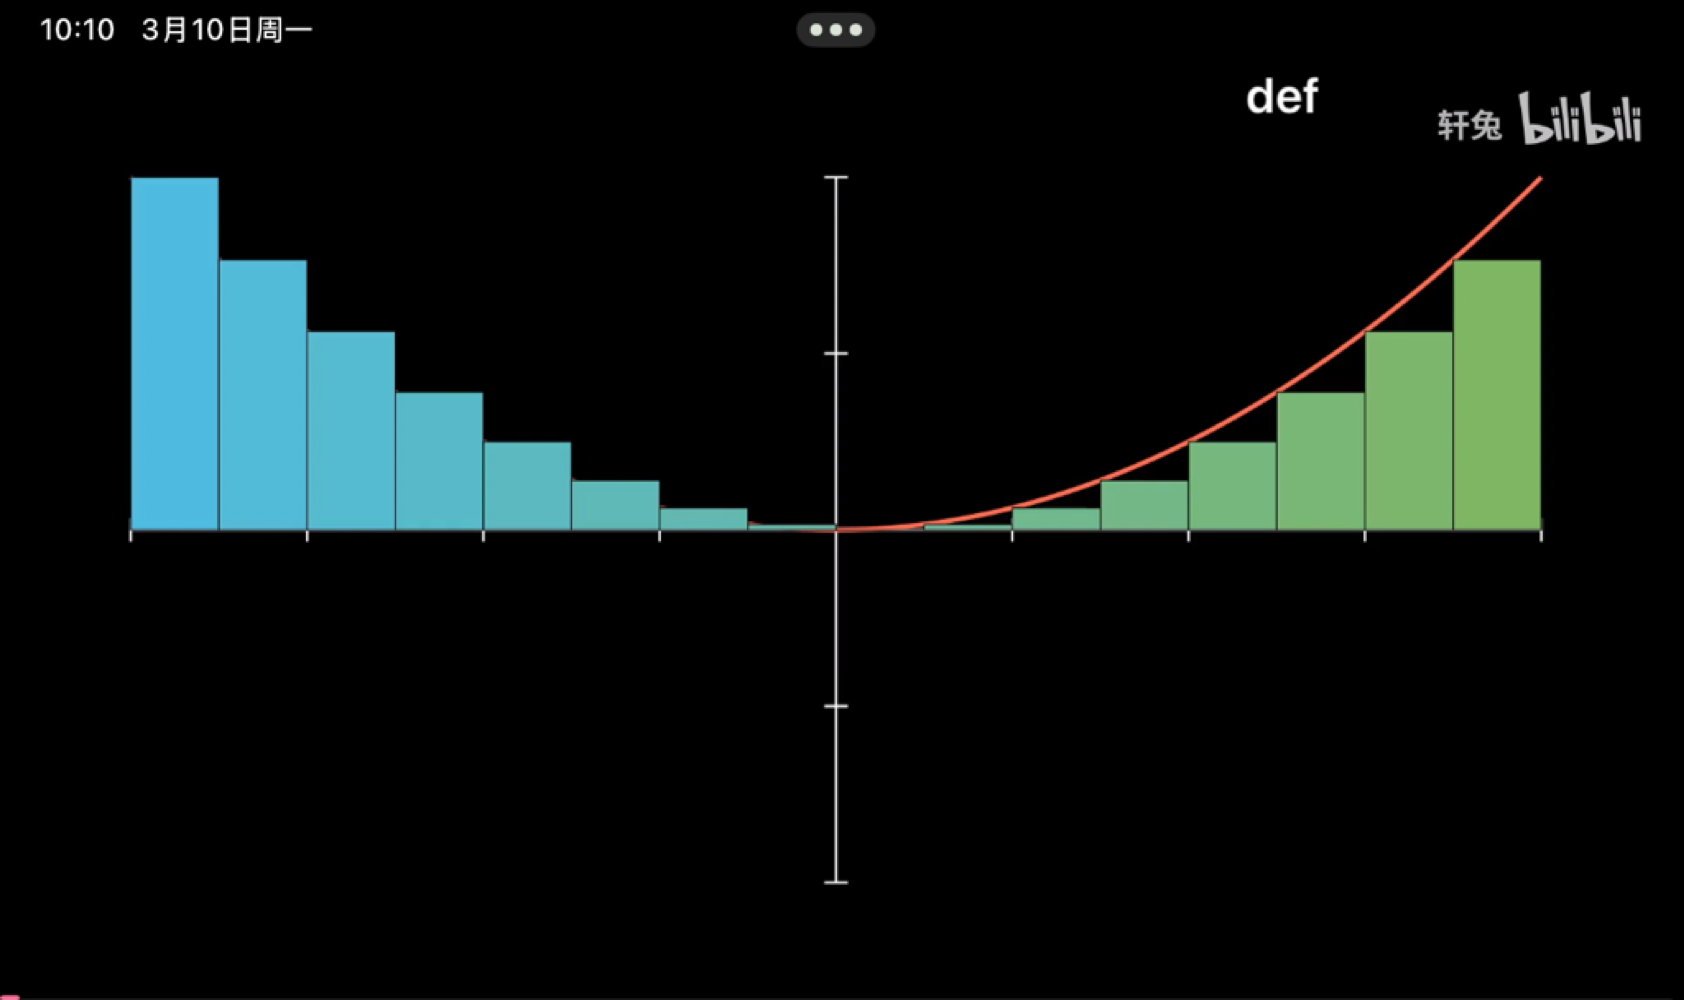
\includegraphics[width=0.5\textwidth]{image/lebegueimage.png}
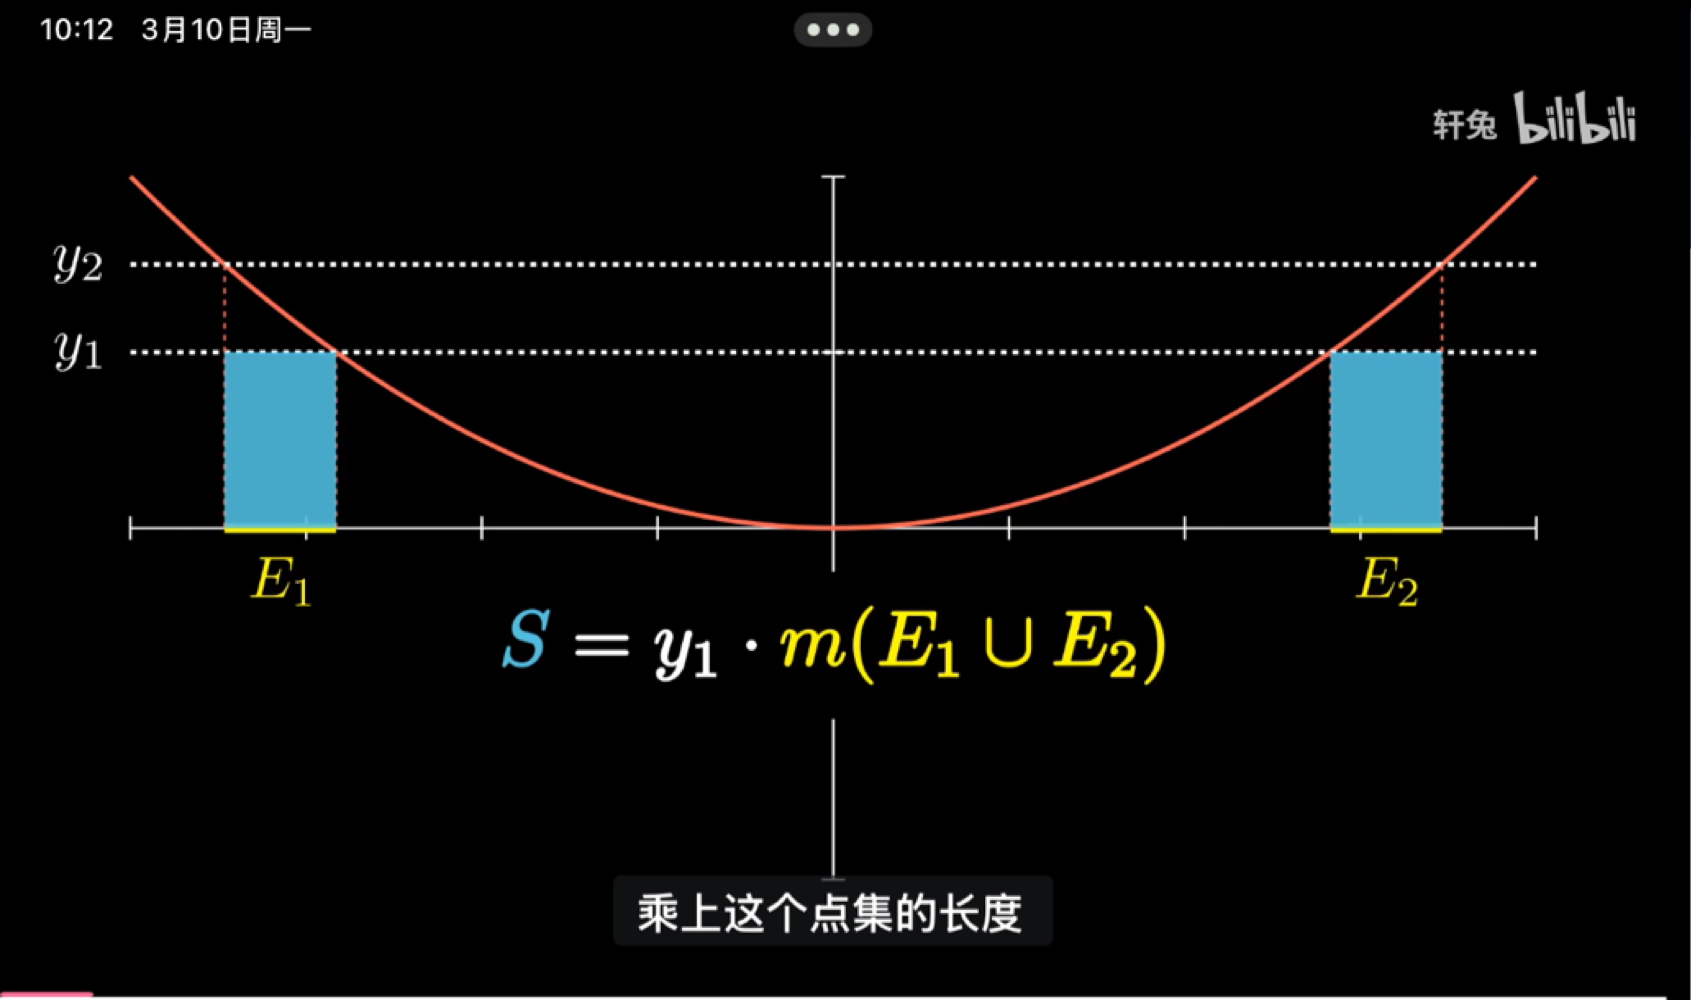
\includegraphics[width=0.5\textwidth]{image/integralimage.png}
学习测度最终的目的是积分,之前黎曼积分如左图是竖着条形我们是用底乘高从左往右积分,是先找到底是多长再找到他对应的高。有一个好处也是我们为什么开始学的是黎曼积分,就是他的底是连续的。而右图lebague积分是先确定了y的区间再确定x的区间,之前是确定自变量在确定因变量,现在是先确定因变量再找对应的自变量。勒贝格积分就不要求自变量是连续的了,如果说黎曼积分自变量是在开区间上定义的,那么勒贝格积分对自变量的要求就是开集了,但是开集也需要良好的性质才能方便测量大小所以引入我们的外测度和测度。
\section{外测度}
\begin{definition}[外测度]\label{def:outermeasure}
设 $E\subset\mathbb{R}^n$,$\{I_k\}_{k=1}^\infty$ 是可数个开矩体,且
\[
\bigcup_{k=1}^\infty I_k\supset E.
\]
则称 $\{I_k\}$ 为 $E$ 的一个 \emph{Lebesgue 覆盖}(简称 $L$-覆盖)。定义
\[
m^*(E)
:=
\inf\Biggl\{\sum_{k=1}^\infty \bigl|I_k\bigr|
  \,\Bigm|\,
  \{I_k\}_{k=1}^\infty \text{ 为 }E\text{ 的 }L\text{-覆盖}
\Biggr\}
\]
为 $E$ 的\emph{外测度}。若 $m^*(E)=0$,则称 $E$ 为\emph{零测集}。
\end{definition}
开矩体就开区间在n维欧氏空间的一般名称,为什么要用矩体来覆盖呢?因为只有不离散的点才能测量长度比如说[0,1]并[2,3]这个集合长度我们怎么测呢测不了,得分别测[0,1]和[2,3]
\begin{theorem}[小矩体 $L$-覆盖]\label{thm:small‐cubes‐cover}
设 $E\subset\mathbb{R}^n$ 且 $m^*(E)<\infty$。则对任意 $\varepsilon>0$,存在 $E$ 的一个小矩体 $L$-覆盖 $\{I_k\}_{k=1}^\infty$,使得
\[
\sum_{k=1}^\infty \lvert I_k\rvert < m^*(E) + \varepsilon,
\qquad
\mathrm{diam}(I_k)<\varepsilon,\quad k=1,2,\dots.
\]
\end{theorem}
这个定理需要例题,我们知道如果要证明两个集合相等最普遍的方式就是他们互相包含,这个小矩体 L覆盖就是干这个的。
\begin{theorem}[外测度的基本性质]\label{thm:outermeasure-basic}
设 \(m^*\) 为 \(\mathbb{R}^n\) 上的外测度,则对任意子集 \(E,E_1,E_2,\dots\subset\mathbb{R}^n\),有:
\begin{enumerate}
  \item[(1)] {\bf 非负性}:
    \[
      \forall E\subset\mathbb{R}^n,\quad
      0\le m^*(E)\le+\infty.
    \]
  \item[(2)] {\bf 单调性}:
    \[
      E_1\subset E_2\subset\mathbb{R}^n
      \quad\Longrightarrow\quad
      m^*(E_1)\le m^*(E_2).
    \]
  \item[(3)] {\bf 次可加性}:
    \[
      m^*\biggl(\bigcup_{k=1}^\infty E_k\biggr)
      \le \sum_{k=1}^\infty m^*(E_k).
    \]
  \item[(4)] {\bf 分离可加性}:若
    \(\displaystyle d(E_1,E_2)
      :=\inf_{\substack{x\in E_1\\y\in E_2}}\|x-y\|>0\),则
    \[
      m^*(E_1\cup E_2)
      = m^*(E_1)+m^*(E_2).
    \]
  \item[(5)] {\bf 平移不变性}:对任意 \(x\in\mathbb{R}^n\),
    \[
      m^*(x+E)=m^*(E).
    \]
  \item[(6)] {\bf 齐次性}:对任意 \(\lambda\neq0\),记
    \(\lambda E=\{\lambda x\mid x\in E\}\),则
    \[
      m^*(\lambda E)=|\lambda|^n\,m^*(E).
    \]
\end{enumerate}
\end{theorem}
平移不变形就像你把椅子从房间搬到客厅,椅子的大小是不变的,齐次性就是你在一维把一条线放大$\lambda$倍\\
他的长度就是原来的$\lambda$倍,但是二维的时候矩形你把每条线都扩大成$\lambda$,面积就变成原来的$\lambda^2$倍。单调性可以与前面的小矩体覆盖联动。看见不等号都应该明白这以后都是放缩的依据。
\begin{definition}[零测集]
    可数点集是零测集
\end{definition}
\begin{center}
    

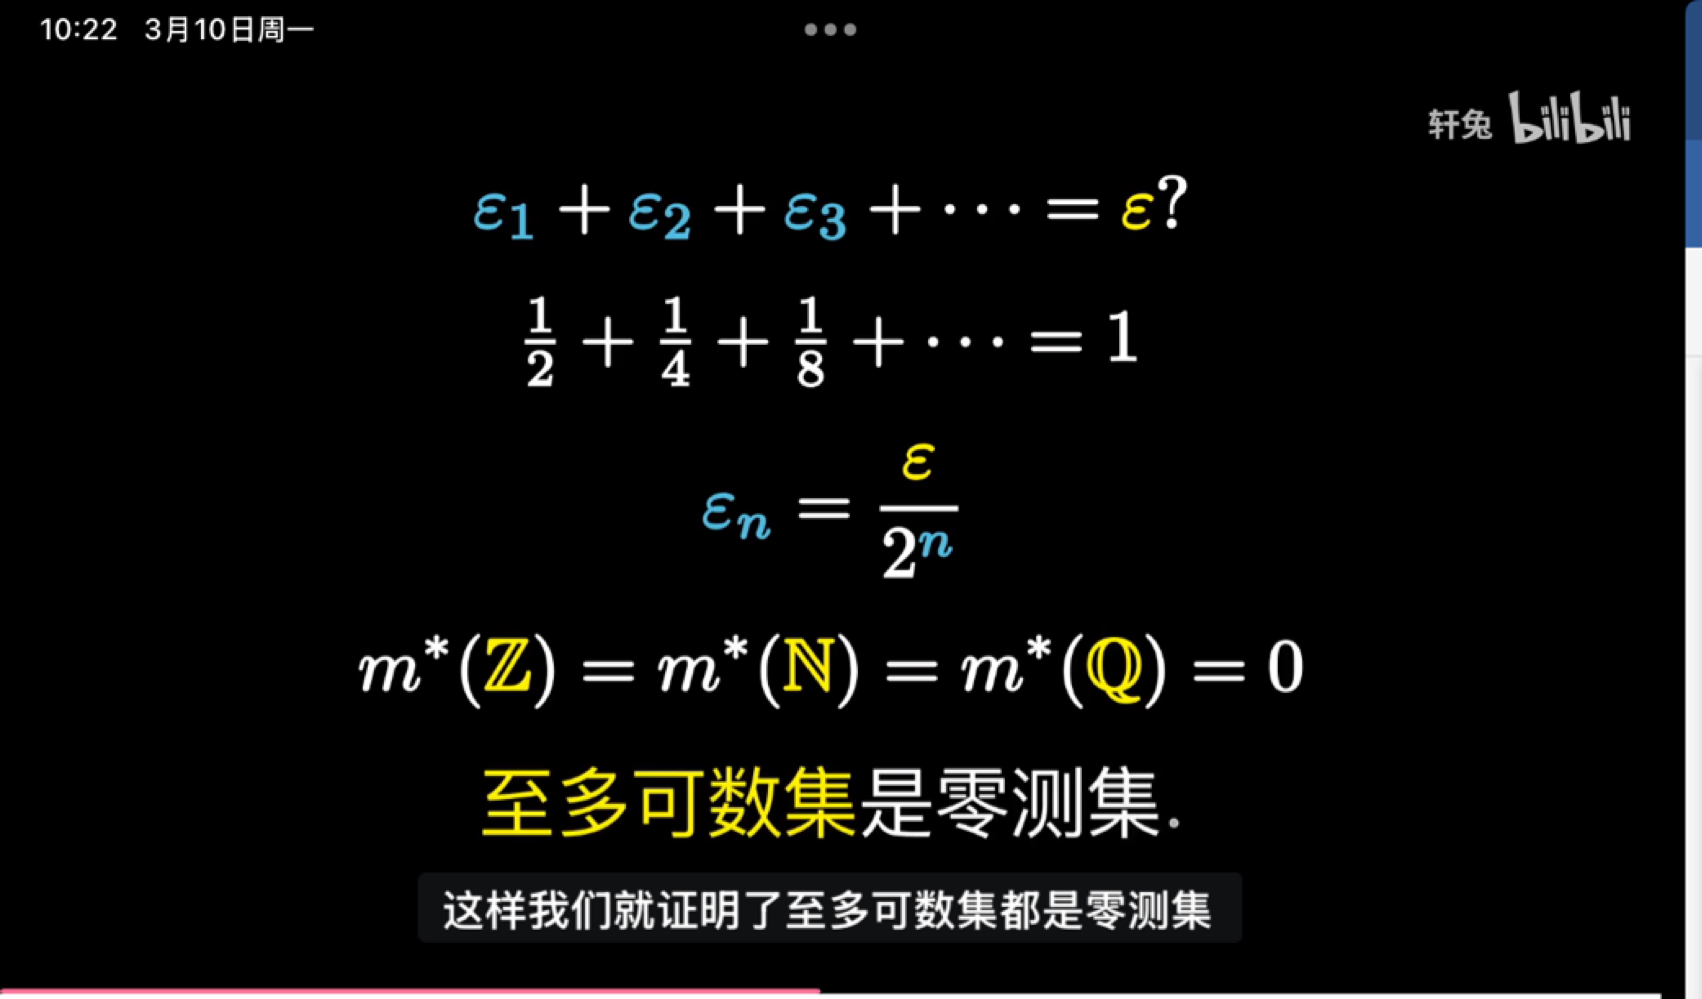
\includegraphics[width=0.5\textwidth]{零测集image.png}
\end{center}
这个图需要谨记,我们构造集合列的可以每一个拓宽 $\epsilon_n$的长度还能保证整体拓展$\epsilon$

\section{外测度与测度}
\begin{center}
    

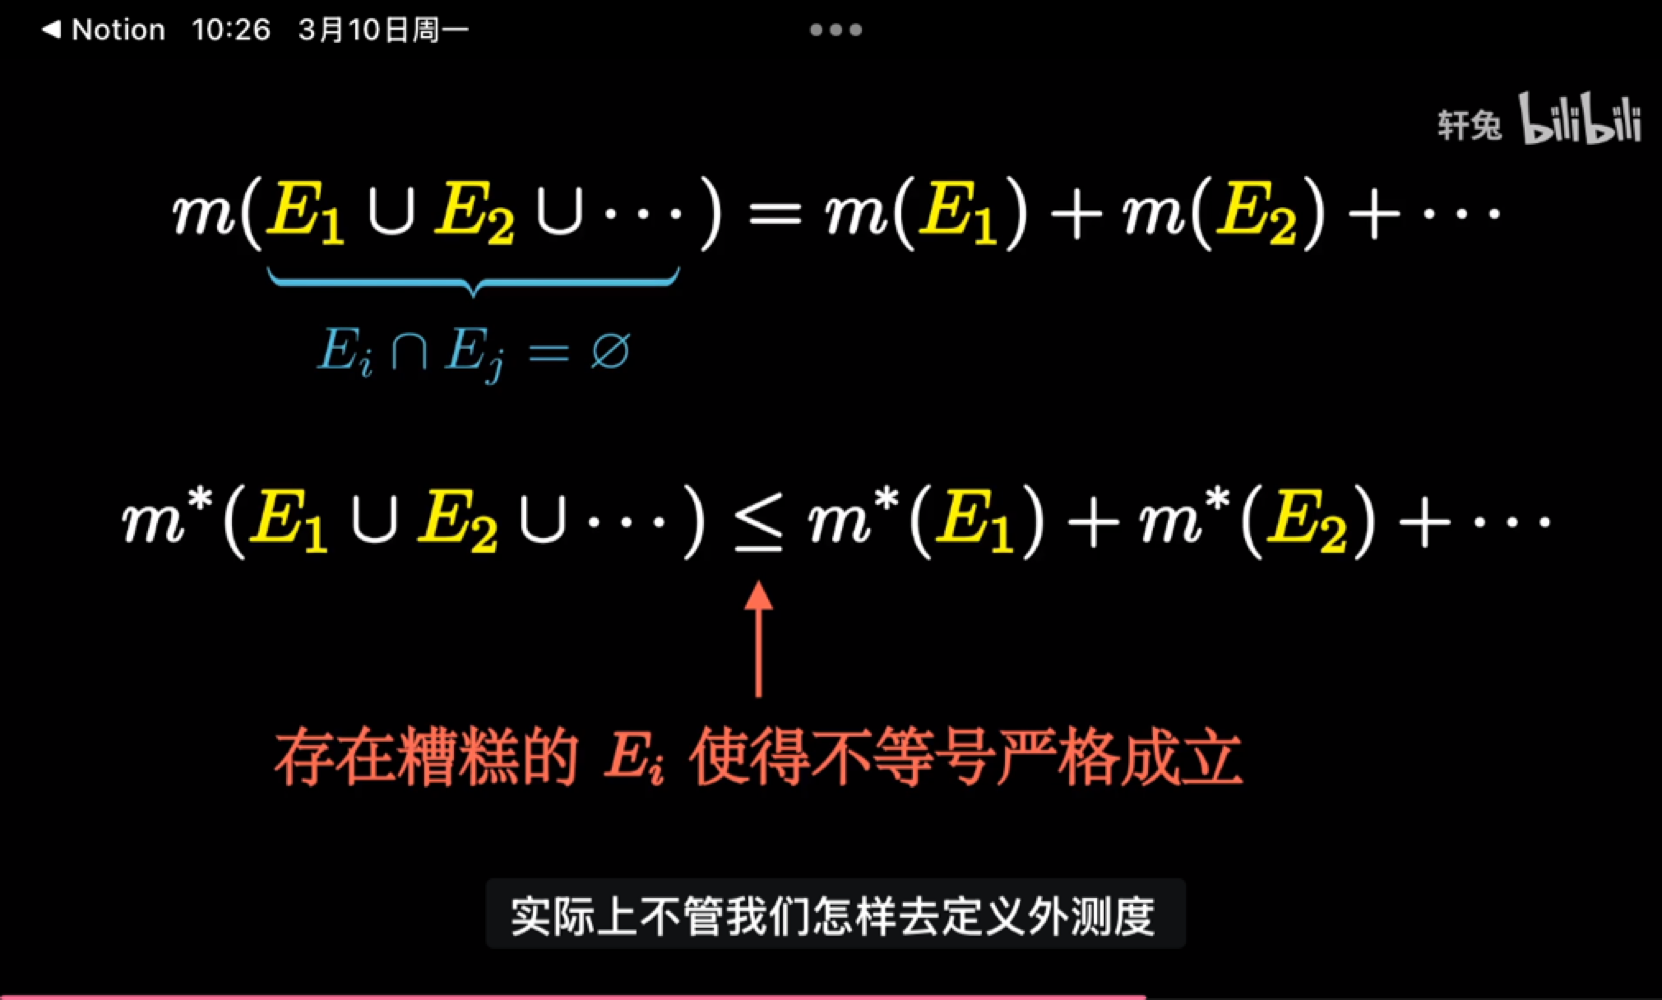
\includegraphics[width=0.5\textwidth]{image/pdf/测度与外测度image.png}
\end{center}
这里有个重点,刚才我们学外测度性质4是分离可加性并不是要求两个集合无交就行而是需要有一定距离。所以如果我们如果像把4的条件拓展的到无交并就要一部分集合踢出去。保留下的集合结构良好我们叫可测集,那些结构不好的就是不可测集。所有集合都有外测度但不是所有集合都是可测得。
\section{可测集}
\begin{definition}[可测集]
设 $E \subset \mathbb{R}^n$,称 $E$ 为一个 \textbf{Lebesgue 可测集}(简称可测集),记为
\[
E \in \mathcal{M} \quad \text{或} \quad E \in \mathcal{M}(\mathbb{R}^n),
\]
如果对任意的矩体 $I \subset \mathbb{R}^n$,有
\[
m^*(I) = m^*(I \cap E) + m^*(I \setminus E).
\]
\end{definition}
我们学习实变函数的时候会频繁的从矩体推广成推广到开集
\begin{theorem}[Carathéodory 条件]
设 $E \subset \mathbb{R}^n$,则 $E$ 是可测集,当且仅当对任意 $T \subset \mathbb{R}^n$,有
\[
m^*(T) = m^*(E \cap T) + m^*(T \setminus E).
\]
\end{theorem}
\begin{theorem}[可测集的可加性]
设 $E \subset \mathbb{R}^n$,则 $E \in \mathcal{M}$ 当且仅当对任意 $A \subset E, \; B \subset E^c$,有
\[
m^*(A \cup B) = m^* A + m^* B.
\]
\end{theorem}

\begin{proof}
必要性:设 $E \in \mathcal{M}$。取 $T = A \cup B$,利用 Carathéodory 条件立即获证。

充分性:$\forall T \subset \mathbb{R}^n$,由于 $E \cap T \subset E$,$T \setminus E \subset E^c$,所以
\[
m^*(T \cap E) + m^*(T \setminus E) = m^*((T \cap E) \cup (T \setminus E)) = m^* T.
\]

这说明 $E \in \mathcal{M}$。
\end{proof}
证明题中可测就可以写出卡拉多利德条件,然后就交并拆括号和括号。
\begin{theorem}[测度的可列可加性]
设 $\{E_k\}_{k \in \mathbb{N}}$ 是一列两两不交的可测集,那么对任意的 $A_k \subset E_k, \; k = 1, 2, \dots$,有
\[
m^*\left( \bigcup_{k=1}^{\infty} A_k \right) = \sum_{k=1}^{\infty} m^* A_k.
\]
\end{theorem}

\begin{proof}
$\forall N \in \mathbb{N}$,有 $A_N \subset E_N$,$\bigcup_{k=1}^{N-1} A_k \subset \bigcup_{k=1}^{N-1} E_k \subset E_N^c$,所以
\[
m^*\left( \bigcup_{k=1}^{N} A_k \right) = m^*\left( \left( \bigcup_{k=1}^{N-1} A_k \right) \cup A_N \right) = m^*\left( \bigcup_{k=1}^{N-1} A_k \right) + m^* A_N.
\]

对 $N$ 作归纳法可得
\[
m^*\left( \bigcup_{k=1}^{N} A_k \right) = \sum_{k=1}^{N} m^* A_k.
\]

于是
\[
\sum_{k=1}^{\infty} m^* A_k = \lim_{N \to \infty} \sum_{k=1}^{N} m^* A_k = \lim_{N \to \infty} m^*\left( \bigcup_{k=1}^{N} A_k \right) \leq m^*\left( \bigcup_{k=1}^{\infty} A_k \right).
\]
\end{proof}
可列的程度还是能保持结构和性质的,证明是可测集的时候常常把外测度的次可加性和单调性当作证明手段。
\begin{theorem}[可测集的可减性]
设 $E_1 \subset E_2 \subset \mathbb{R}^n$,若 $E_1 \in \mathcal{M}$ 且 $m E_1 < \infty$,则
\[
m^*(E_2 \setminus E_1) = m^* E_2 - m^* E_1.
\]
\end{theorem}
\begin{theorem}[可测对集合运算的封闭性]
\begin{enumerate}
  \item 若 $E \in \mathcal{M},\ x \in \mathbb{R}^n,\ \lambda \neq 0$,则 $E^c,\ x + E,\ \lambda E \in \mathcal{M}$;
  
  \item 若 $E_1, E_2 \in \mathcal{M}$,则 $E_1 \cup E_2,\ E_1 \cap E_2,\ E_1 \setminus E_2 \in \mathcal{M}$;
  
  \item 若 $E_1, E_2, \dots \in \mathcal{M}$,则
  \[
  \bigcup_{k=1}^{\infty} E_k,\quad \bigcap_{k=1}^{\infty} E_k,\quad \lim_{k \to \infty} E_k,\quad \overline{\lim_{k \to \infty}} E_k \in \mathcal{M}.
  \]
\end{enumerate}
\end{theorem}
可测集的“可测性”本质上描述了一种 \textbf{与外测度兼容的分割性质}。具体而言,对于集合 $E$,若对任意集合 $A \subset \mathbb{R}^n$,都有
\[
m^*(A) = m^*(A \cap E) + m^*(A \cap E^c),
\]
则称 $E$ 是一个 \textbf{可测集},记作 $E \in \mathcal{M}$。

这个定义的核心思想是,外测度在 $E$ 和其补集 $E^c$ 上能\textbf{无缝地分解},没有测度上的“重叠”或“缺口”。

由此可以得到如下直观理解:
\begin{itemize}
  \item 可测性与集合是否有限无关。一个集合即使测度为 $\infty$,也可能是可测的。
  \item 若 $E$ 是可测的,则其补集 $E^c$ 也是可测的。这是由于定义在 $E$ 与 $E^c$ 上是对称的。
  \item 有限个可测集的并、交、差仍是可测集。即集合族 $\mathcal{M}$ 在这些运算下封闭。
  \item 因此,\textbf{“属于 $\mathcal{M}$” 就是“是可测集”的意思}。
\end{itemize}
\section{可测集的构造}
\begin{theorem}
    零测集是可测集
\end{theorem}
我们数学中常常有+0-0的操作,零测集也是这个用法而且零测集很好构造,特别在逼近领域常常用到。
\begin{corollary}
    开集闭集都是可测集
\end{corollary}
这给我们证明一个集合是可测集又提供了思路。
\begin{theorem}
任何矩体 $I$(无论它是开、闭或部分开部分闭的)均可测,且
\[
mI = |I|.
\]
\end{theorem}
\begin{theorem}[可测集可用开集和闭集逼近]
设 $E \in \mathcal{M}$,则对任意 $\varepsilon > 0$,存在开集 $G$ 和闭集 $F$,满足
\[
F \subset E \subset G, \quad \text{且} \quad m(G \setminus E) < \varepsilon, \quad m(E \setminus F) < \varepsilon.
\]
\end{theorem}
\begin{proof}
先考虑 $mE < \infty$ 的情形。
\textcolor{red}{我们希望证明:$E$ 和某个开集 $G$ 的差在测度意义上非常小,即 $m(G \setminus E) < \varepsilon$,这意味着 $E$ 与 $G$ 的“差距”可以忽略,从测度的角度讲它们“几乎一样”。}

对任意 $\varepsilon > 0$,取 $E$ 的一个 $\mathcal{L}$-覆盖 $\{I_k\}_{k=1}^\infty$,使得
\[
\sum_{k=1}^\infty |I_k| < mE + \varepsilon.
\]
记 $G := \bigcup_{k=1}^\infty I_k$,则 $G$ 是一个开集,$G \supset E$,且
\[
mG \leq \sum_{k=1}^\infty |I_k| < mE + \varepsilon.
\]
因此有
\[
m(G \setminus E) = mG - mE < \varepsilon.
\]

\vspace{1em}
接下来考虑 $mE = \infty$ 的情形。
\textcolor{red}{我们将无限测度问题转化为有限测度问题来处理:}

\begin{itemize}
  \item 
  \textcolor{red}{首先将 $E$ 拆成若干个测度有限的部分:}取一列有界集合 $\{B_k\}_{k \in \mathbb{N}}$,使得
  \[
  \bigcup_{k=1}^\infty B_k = \mathbb{R}^n,
  \]
  \textcolor{red}{例如可以令 $B_k = [-k, k]^n$。n维矩体}
  
  \item 记 $E_k := E \cap B_k$,则 $E = \bigcup_{k=1}^\infty E_k$,且每个 $E_k$ 都是测度有限的。
\end{itemize}

对每个 $k$,由有限测度情形,存在开集 $G_k \supset E_k$,满足
\[
m(G_k \setminus E_k) < \frac{\varepsilon}{2^k}.
\]
\textcolor{red}{这里将 $\varepsilon$ 按等比数列分配,是为了确保级数 $\sum \varepsilon/2^k$ 收敛,从而最终的测度误差控制在 $\varepsilon$ 以内。}

设
\[
G := \bigcup_{k=1}^\infty G_k,
\]
则 $G$ 是开集,$G \supset E$,且
\[
\begin{aligned}
m(G \setminus E)
&= m\left( \bigcup_{k=1}^\infty (G_k \setminus E) \right)
\leq \sum_{k=1}^\infty m(G_k \setminus E) \\
&\leq \sum_{k=1}^\infty m(G_k \setminus E_k)
< \sum_{k=1}^\infty \frac{\varepsilon}{2^k} = \varepsilon.
\end{aligned}
\]

对 $E^c$,利用同样的方法可得存在开集 $G_1 \supset E^c$,使得 $m(G_1 \setminus E^c) < \varepsilon$。

设 $F := G_1^c$,则 $F$ 是闭集,$F \subset E$,且
\[
m(E \setminus F) = m(G_1 \setminus E^c) < \varepsilon.
\]
\end{proof}
\begin{definition}[$G_\delta$ 型集、$F_\sigma$ 型集]
$\mathbb{R}^n$ 中可列个开集的交称为 $G_\delta$ 型集,可列个闭集的并称为 $F_\sigma$ 型集。
\end{definition}

下面的定理彻底解决了可测集的构造问题。它说明可测集其实就是零测集与开集或闭集的可数运算所形成的。

\begin{corollary}
设 $E \subset \mathbb{R}^n$,则 $E \in \mathcal{M}$ 与如下任意一条等价:
\begin{itemize}
  \item[(i)] 对任意 $\varepsilon > 0$,存在开集 $G \supset E$,使得 $m^*(G \setminus E) < \varepsilon$;
  \item[(ii)] 对任意 $\varepsilon > 0$,存在闭集 $F \subset E$,使得 $m^*(E \setminus F) < \varepsilon$;
  \item[(iii)] 存在 $G_\delta$ 型集 $G \supset E$,使得 $m^*(G \setminus E) = 0$;
  \item[(iv)] 存在 $F_\sigma$ 型集 $F \subset E$,使得 $m^*(E \setminus F) = 0$。
\end{itemize}
\end{corollary}
\begin{theorem}[可测集的构造]
设 $E \in \mathcal{M}$,则存在 $F_\sigma$ 型集 $F$ 和 $G_\delta$ 型集 $G$,满足
\[
F \subset E \subset G, \quad \text{且} \quad m(G \setminus E) = m(E \setminus F) = 0.
\]
从而,
\[
E = G \setminus N_1 = F \cup N_2,
\]
其中 $N_1, N_2$ 均为零测集。
\end{theorem}

\begin{theorem}[乘积集合的可测性]
设 $E_1, E_2$ 分别是 $\mathbb{R}^n, \mathbb{R}^m$ 中可测集,其中 $n, m \in \mathbb{N}$,则
\[
E_1 \times E_2 := \{(x, y) \mid x \in E_1,\, y \in E_2\}
\]
是 $\mathbb{R}^{n+m}$ 中的可测集,且
\[
m(E_1 \times E_2) = mE_1 \times mE_2.
\]
\end{theorem}
这一定理是后续 Fubini 定理 和 Tonelli 定理 的基础,说明了可测集在乘积空间中也保持可测性,且测度具有乘法性。






\section{不可测集}
\begin{definition}[不可测集]
    不可测集的经典构造vital集
\end{definition}
\textbf{Vitali 集的构造与不可测性证明}

在区间 $[0,1]$ 上定义如下等价关系:
\[
x \sim y \iff x - y \in \mathbb{Q}, \quad x,y \in [0,1].
\]
显然,这是一个等价关系,它将 $[0,1]$ 划分为若干个不交的等价类。每个等价类中的所有元素之间的差是有理数。

由于 $\mathbb{Q}$ 是可数集,而 $[0,1]$ 是不可数的,所以存在不可数个这样的等价类。现在,\textbf{使用选择公理},从每一个等价类中任意选取一个代表元,构成一个集合 $V$,称为 \textbf{Vitali 集}。

\[
V = \{ \text{每个等价类中选取的一个元素} \} \subset [0,1].
\]

考虑所有的有理数 $q \in \mathbb{Q} \cap [-1,1]$,并将 $V$ 按这些有理数平移,记:
\[
V_q = V + q = \{ v + q : v \in V \}.
\]

记住:如果 $q_1 \ne q_2$,则 $V_{q_1} \cap V_{q_2} = \varnothing$。原因如下:

- 若 $x \in V_{q_1} \cap V_{q_2}$,则存在 $v_1, v_2 \in V$ 使得 $x = v_1 + q_1 = v_2 + q_2$;
- 于是 $v_1 - v_2 = q_2 - q_1 \in \mathbb{Q}$,说明 $v_1 \sim v_2$;
- 但 $v_1, v_2 \in V$ 且来自不同代表元集合,矛盾。

因此,这些平移后的集合 $\{V_q\}_{q \in \mathbb{Q} \cap [-1,1]}$ 是两两不交的。

另一方面,注意到这些集合的并至少覆盖了 $[0,1]$:
\[
[0,1] \subset \bigcup_{q \in \mathbb{Q} \cap [-1,1]} V_q \subset [-1,2].
\]

设想 $V$ 是一个 Lebesgue 可测集,记 $m(V)$ 为其测度。那么,由于 Lebesgue 测度在平移下保持不变,有:
\[
m(V_q) = m(V), \quad \forall q \in \mathbb{Q} \cap [-1,1].
\]

而 $\{V_q\}$ 两两不交,因此:
\[
\sum_{q \in \mathbb{Q} \cap [-1,1]} m(V_q) = \sum_{q \in \mathbb{Q} \cap [-1,1]} m(V).
\]

由于 $\mathbb{Q} \cap [-1,1]$ 是可数无穷集,这个和为:
- 若 $m(V) > 0$,则总和为 $\infty$,矛盾,因为这些集合的并包含于 $[-1,2]$,测度至多为 $3$;
- 若 $m(V) = 0$,则并集测度为 $0$,矛盾,因为它覆盖了 $[0,1]$,测度为 $1$。

综上,$V$ 无法具有一致的 Lebesgue 测度,因此 \textbf{Vitali 集 $V$ 不是 Lebesgue 可测集}。
\chapter{第三章可测函数}
\section{可测函数封闭性}
\begin{definition}
设 $E \subset \mathbb{R}^n$ 可测,若对任意 $a \in \mathbb{R}$,有 $\{x \in E \mid f(x) > a\} \in \mathcal{M}$,则称 $f$ 为 $E$ 上的 \textbf{Lebesgue 可测函数},简称为可测函数。
\end{definition}
可测函数本质这个定义就是f的原像集可测,我们要多用映射这个概念,函数就是两个集合之间的映射比如y=x实数范围内 就是一个实数集到另一个实数集到映射,他们中的元素存在一一对应关系。原像就是x,像就是y。
\begin{theorem}[可测函数的等价表述]
设 $f$ 是可测集 $E$ 上的函数,则 $f$ 可测当且仅当下列之一成立:
\begin{enumerate}
  \item 对任意 $a \in \mathbb{R}$,有 $\{x \in E \mid f(x) > a\} \in \mathcal{M}$;
  \item 对任意 $a \in \mathbb{R}$,有 $\{x \in E \mid f(x) < a\} \in \mathcal{M}$;
  \item 对任意 $a \in \mathbb{R}$,有 $\{x \in E \mid f(x) \leq a\} \in \mathcal{M}$。
\end{enumerate}
\end{theorem}
\begin{definition}
设 $P(x)$ 是可测集 $E \subset \mathbb{R}^n$ 上的一个命题,若
\[
\{x \in E \mid P(x) \text{ 不成立} \}
\]
是一个零测集,则称 $P(x)$ 在 $E$ 上\textbf{几乎处处成立},记作
\[
P(x) \text{ a.e. } x \in E.
\]
\end{definition}

几乎处处是一个非常重要的定理,说明了只要不符合要求的是零测集就不影响性质,很多题目也是要求几乎处处就行了。a,e almost everywhere,学习数学把定理的英文名称搜索一下会很有帮助。

\begin{theorem}[几乎处处相等的函数具有相同的可测性]
若 $f, g$ 均为 $E$ 上函数,$f$ 可测,且 $f(x) = g(x)$ a.e. $x \in E$,则 $g$ 也是 $E$ 上可测函数。
\end{theorem}

\begin{proof}
记 $E_0 := \{x \in E \mid f(x) \neq g(x)\}$,则 $E_0$ 是一个零测集,因而 $g$ 是 $E_0$ 上可测函数。

而 $g$ 在 $E \setminus E_0$ 上恒等于可测函数 $f$,所以 $g$ 在 $E \setminus E_0$ 上也可测。

根据定理 3.1.2,$g$ 在 $E = E_0 \cup (E \setminus E_0)$ 上可测。
\end{proof}

\begin{theorem}[函数可测性对算术运算的封闭性]
设 $f, g$ 是 $E$ 上可测函数,$c \in \mathbb{R}$,则
\[
cf,\quad |f|,\quad f + g,\quad fg,\quad \frac{f}{g},\quad \min(f, g),\quad \max(f, g)
\]
均为 $E$ 上可测函数(假设所进行的运算在 $E$ 上几乎处处有意义)。
\end{theorem}
\begin{theorem}[函数可测性对极限运算的封闭性]
设 $\{f_k\}_{k=1}^\infty$ 为 $E$ 上一列可测函数,则
\[
\sup_{k \in \mathbb{N}} f_k,\quad \inf_{k \in \mathbb{N}} f_k,\quad \limsup_{k \to \infty} f_k,\quad \liminf_{k \to \infty} f_k
\]
均为 $E$ 上可测函数。
\end{theorem}
\section{从简单函数到一般函数}
正如无数次我们需要从特殊到一般,这次我们仍然需要从特殊大简单函数了解他的性质然后进行推广。
\begin{definition}[简单函数]
设 $f$ 是 $E \in \mathcal{M}$ 上的函数,如果 $E$ 可分解为有限个互不相交的可测集的并:
\[
E = \bigcup_{k=1}^{N} E_k, \quad E_i \cap E_j = \emptyset, \ \forall i \ne j,
\]
使得 $f$ 在每一个 $E_k$ 上为实常数(不为 $\pm \infty$),则称 $f$ 为 $E$ 上的简单函数。
\end{definition}

简单函数可以看作一种分段常数函数。与初等分段函数(如 $y=1$ 当 $x>0$,$y=-1$ 当 $x \leq 0$)不同,简单函数允许每一段的定义域由多个区间甚至非连续集合构成,例如 $f(x) = 1$ 当 $x \in A$,其中 $A$ 是形如 $(0,1) \cup (1.5, 2.5)$ 的集合。这样可以更方便、简洁地表示复杂的定义域结构。
我们验证一下简单函数是可测的,即E(f>a)可测,这个原像集也是有限个互补相交的可测集的并,所以用可测集的封闭性可以知道原像集也是可测的。注意如果是不可数个可测集的并是可以形成不可测集的。
\begin{definition}{特征函数}
    特征函数这种书写方式让我们对x是在哪个集合有效也就是x=1很直观也就是下角标$E_k$

在可测集 $E$ 上的简单函数可以写成有限个特征函数的线性组合:
\[
f(x) = \sum_{k=1}^{N} c_k \chi_{E_k}(x), \quad \forall x \in E,
\]
其中 $c_k$ 表示 $f$ 在 $E_k$ 上的取值,$\chi_{E_k}$ 表示集合 $E_k$ 的特征函数,即
\[
\chi_{E_k}(x) =
\begin{cases}
1, & x \in E_k, \\
0, & x \in \mathbb{R}^n \setminus E_k.
\end{cases}
\]
\end{definition}
$\chi$是希腊字符 叫chi 谐音是开“chi” 来自单词 characteristic(特征),如果不明白某一个名字的意思还是去找他的英文单词比较好。
定义在不可测集上的函数当然不可测。
但是定义在可测集上的函数也有可能不可测。\\
我们可以通过不可测集合构造一个不可测函数。
\begin{enumerate}
  \item 构造一个不可测集合 $V \subseteq [0,1]$,例如 \emph{Vitali 集合}。
  
  \item 定义函数 $f: [0,1] \to \mathbb{R}$ 为:
  \[
  f(x) = 
  \begin{cases}
  1, & x \in V, \\
  0, & x \in [0,1] \setminus V.
  \end{cases}
  \]
\end{enumerate}

注意:
\begin{itemize}
  \item 该函数的定义域是可测集 $[0,1]$;
  \item 但函数 $f$ 是不可测的,因为集合 $V$ 是不可测集合,导致集合 $\{x \in [0,1] \mid f(x) > 0.5\} = V$ 不是可测集;
  \item 所以函数 $f$ 不满足勒贝格可测函数的定义。
\end{itemize}
\begin{lemma}[简单函数封闭性]
设 $\phi_1, \phi_2$ 均为集合 $E \subset \mathbb{R}^n$ 上简单函数,$c \in \mathbb{R}$,则 $c\phi_1, \phi_1 + \phi_2, \phi_1\phi_2$ 也是 $E$ 上简单函数。
\end{lemma}

\begin{theorem}[可测函数是简单函数的极限]
设 $f$ 是 $E$ 上的可测函数,则:

\begin{enumerate}[(1)]
    \item 若 $f$ 是 $E$ 上的非负可测函数,则存在渐升的非负简单函数列 $\{\varphi_k\}$,使得
    \[
    f(x) = \lim_{k \to \infty} \varphi_k(x), \quad \forall x \in E.
    \]

    \item 若 $f$ 是 $E$ 上的可测函数,则存在简单函数列 $\{\varphi_k\}_{k=1}^\infty$,满足
    \[
    |\varphi_k(x)| \leq |f(x)|, \quad \text{且} \quad f(x) = \lim_{k \to \infty} \varphi_k(x), \quad \forall x \in E.
    \]
\end{enumerate}
date 2025.8.5\\
在上述两种情形中,若 $f$ 有界,那么收敛是一致的。
\end{theorem}
在构造可测函数 $f$ 的简单函数逼近时,引入“非负”和“渐升”的条件,是为了使用单调极限逼近,必须非负才能用“单调收敛定理”,确保极限存在。我们这样才可以构造出一列简单函数
 。$\{\varphi_k\}$,使得它们逐点极限收敛于 $f$,即:
\[
\lim_{k \to \infty} \varphi_k(x) = f(x), \quad \forall x \in E,
\]
并且对于任意 $\varepsilon > 0$,存在正整数 $K$,当 $k \geq K$ 时,有
\[
|f(x) - \varphi_k(x)| < \varepsilon, \quad \forall x \in E.
\]
下面是一种经典构造方法


\textbf{证}\quad $\forall k \in \mathbb{N}$,记
\[
E_{k,j} := 
\begin{cases}
E\left( \dfrac{j}{2^k} \leq f < \dfrac{j+1}{2^k} \right), & j = 0, 1, \dots, k2^k - 1, \\
E(f \geq k), & j = k2^k.
\end{cases}
\]
这个构造方法也是数学核心思想,把无限分成有限+有条件的无限。这里(1)中并没有限制f的值域所以我们要讨论他的值域趋紧无穷大的情况。第一部分把有限的部分不断细分且扩大原像集,第二个部分大于k的部分始终取值为k。
分割的程度也和k有关因为j的最大值就是k$2^k$-1,可以看作j是$E_k$的序号。看清每一个下标是什么意思。
\begin{itemize}
   \textbf{具体解释 $j$ 的取值:}
  \begin{itemize}
    \item 我们将区间 $[0, k)$ 分成 $k \cdot 2^k$ 个长度为 $\frac{1}{2^k}$ 的小区间;
    \item 所以 $j = 0, 1, 2, \dots, k2^k - 1$ 就是这些区间的编号;
    \item 对于每个 $j$,构造集合:
    \[
    E_{k,j} := E\left( \frac{j}{2^k} \leq f < \frac{j+1}{2^k} \right)
    \]
    表示函数值落在该小区间的那些点的集合。
  \end{itemize}
  
   \textbf{那为什么最后还要加上 $j = k2^k$ 这一项?}
  \begin{itemize}
    \item 因为我们只把 $f \in [0, k)$ 这部分划分好了;
    \item 若某些 $x \in E$ 上的 $f(x) \geq k$,就会超出这个划分;
    \item 所以我们单独把 $f(x) \geq k$ 的部分拿出来构造成一个额外的集合:
    \[
    E(f \geq k) \quad \text{对应} \quad j = k2^k
    \]
    相当于用一个“兜底项”处理大于等于 $k$ 的部分。
  \end{itemize}
\end{itemize}
\[
E = \bigcup_{j=0}^{k 2^k} E_{k,j}, \quad E_{k,j} \cap E_{k,i} = \varnothing, \quad \forall i \ne j; \quad i,j = 0,1,\dots,k 2^k.
\]

定义 $E$ 上函数 $\varphi_k$ 如下:
\[
\varphi_k(x) := \frac{j}{2^k}, \quad \forall x \in E_{k,j}, \quad j = 0,1,\dots,k 2^k.
\]

显然,$\varphi_k$ 是 $E$ 上非负简单函数。
这和我们开始学微积分的时候达布小和是一样的,用函数值的左端点进行近似。这样当k趋紧于无穷的时候,小于k的部分全部被划分为1/$2^k$值域内近似取左端点不影响,大于k的部分都取的是无穷也符合。
显然 $\varphi_k$ 是 $E$ 上非负简单函数。我们证明:$\forall x \in E$,有
\begin{itemize}
    \item[(a)] $\varphi_k(x) \leq \varphi_{k+1}(x), \quad \forall k \in \mathbb{N};$
    \item[(b)] $\lim\limits_{k \to \infty} \varphi_k(x) = f(x)$.
\end{itemize}

事实上,由 $x \in E$ 可知,$\exists j \in \mathbb{N}: 0 \leq j \leq k2^k$,使得 $x \in E_{k,j}$. 此时,$\varphi_k(x) = \dfrac{j}{2^k}$.

(i) 若 $j \leq k2^k - 1$,则
\[
\frac{j}{2^k} \leq f(x) < \frac{j+1}{2^k},
\]
从而
\[
\frac{2j}{2^{k+1}} \leq f(x) < \frac{2j+1}{2^{k+1}} \quad \text{或} \quad \frac{2j+1}{2^{k+1}} \leq f(x) < \frac{2j+2}{2^{k+1}},
\]
即 $x \in E_{k+1,2j}$ 或 $x \in E_{k+1,2j+1}$。由于 $2j+1 \leq 2(k2^k - 1) + 1 < (k+1)2^{k+1} - 1$,所以
\[
\varphi_{k+1}(x) = \frac{2j}{2^{k+1}} \quad \text{或} \quad \frac{2j+1}{2^{k+1}}.
\]把原来f的取值范围分成两半,f的值总在其中一半。\\
从而 $\varphi_{k+1}(x) \geq \dfrac{j}{2^k} = \varphi_k(x)$。

(ii) 若 $j = k2^k$,则 $\varphi_k(x) = k$,此时 $f(x) \geq k = \dfrac{k2^{k+1}}{2^{k+1}}$。

于是存在 $l \geq k2^{k+1}$,使得 $x \in E_{k+1, l}$。

于是 $\varphi_{k+1}(x) = \dfrac{l}{2^{k+1}} \geq \dfrac{k2^{k+1}}{2^{k+1}} = k = \varphi_k(x)$。

综含 (i)(ii), (a) 得证。下面证 (b)。
若 $f(x)<\infty$,取自然数 $N \geq f(x)$,则当 $k > N$ 时,有 $0 < f(x) < k$,于是存在
$0 \leq j \leq k2^k -1$,使得 $x \in E_{k,j}$,从而
\[
\frac{j}{2^k} \leq f(x) < \frac{j+1}{2^k}, \quad \varphi_k(x) = \frac{j}{2^k},
\]
所以
\[
0 \leq f(x) - \varphi_k(x) < \frac{1}{2^k},
\]
故 $\lim_{k \to \infty} \varphi_k(x) = f(x)$。

若 $f(x) = \infty$,则 $\forall k \in \mathbb{N}$,有 $f(x) > k$,从而 $\varphi_k(x) = k$,所以
\[
\lim_{k \to \infty} \varphi_k(x) = \infty = f(x).
\]
(b) 得证。

当 $f$ 有界时,可以取与 $x$ 无关的 $N$ 满足 $N \geq f(x)$,$\forall x \in E$,所以收敛性结论 (b) 是一致成立的。至此,(1) 获证。
下面证明 (2)。将 $f$ 分解为 $f = f^+ - f^-$。利用 (1) 得,存在渐升的非负简单函数列 $\{\varphi_k\}$ 和 $\{\psi_k\}$,使得
\[
\lim_{k \to \infty} \varphi_k(x) = f^+(x), \quad \lim_{k \to \infty} \psi_k(x) = f^-(x), \quad \forall x \in E.
\]

由引理 3.2.1 可知,$\{\varphi_k - \psi_k\}$ 为 $E$ 上一列简单函数,满足
\[
|\varphi_k(x) - \psi_k(x)| \leq \varphi_k(x) + \psi_k(x) \leq f^+(x) + f^-(x) = |f(x)|, \quad \forall x \in E,
\]
且
\[
\lim_{k \to \infty} [\varphi_k(x) - \psi_k(x)] = f(x), \quad \forall x \in E.
\]

当 $f$ 有界时,由于 $f^+, f^-$ 都是有界的,所以收敛是一致的。
\begin{definition}
设 $f$ 是集合 $E \subset \mathbb{R}^n$ 上的一个实函数,定义 $f$ 的正部与负部如下:
\[
f^+(x) := 
\begin{cases}
f(x), & f(x) \geq 0, \\
0,    & f(x) < 0,
\end{cases}
\qquad
f^-(x) := 
\begin{cases}
0,    & f(x) \geq 0, \\
-f(x), & f(x) < 0.
\end{cases}
\]

即 $f^+$ 表示 $f$ 的正部分,$f^-$ 表示 $f$ 的负部分。

由定义可得:
\[
f^+(x) = \max(f(x), 0), \qquad f^-(x) = -\min(f(x), 0),
\]
并且满足以下关系:
\[
f(x) = f^+(x) - f^-(x), \qquad |f(x)| = f^+(x) + f^-(x).
\]

当 $f$ 是 $E$ 上的可测函数时,$f^+$ 和 $f^-$ 亦为 $E$ 上的可测函数。
\end{definition}
\begin{theorem}[Lusin]
设 $f$ 是 $E \subset \mathbb{R}^n$ 上几乎处处有限的可测函数,则对任意 $\varepsilon > 0$,存在闭集 $F \subset E$,使得
\[
m(E \setminus F) < \varepsilon,
\]
且 $f$ 在 $F$ 上连续。
\end{theorem}

可测+几乎处处有限在一个闭集和原集合差一个零测集 测度差任意小上连续
\begin{theorem}
设 $f$ 是 $E \subset \mathbb{R}^n$ 上几乎处处有限的可测函数,则对任意 $\varepsilon > 0$,存在 $\mathbb{R}^n$ 上连续函数 $g$,使得
\[
m(E(f \neq g)) < \varepsilon, \quad \text{且} \quad \operatorname{supp} g \subset \left\{ x \in \mathbb{R}^n \,\middle|\, d(x, \operatorname{supp} f) \leq \varepsilon \right\}.
\]
此外,若存在常数 $M$ 使得 $|f(x)| < M, \, \forall x \in E$,那么 $g$ 满足 $|g(x)| < M, \, \forall x \in \mathbb{R}^n$。
\end{theorem}
\text{设 } g : \mathbb${R}^n$ \to \mathbb{R},\text{则其支集定义为:}
\[
\operatorname{supp} g := \overline{\{ x \in \mathbb{R}^n \mid g(x) \neq 0 \}}
\]
\text{即 } g \text{不为零的区域的闭包。}
\begin{theorem}[3.2.4 可测函数是连续函数的极限]
设 $f$ 是 $E \subset \mathbb{R}^n$ 上几乎处处有限的可测函数,则存在 $\mathbb{R}^n$ 上连续函数列 $\{f_k\}$,满足
\[
\operatorname{supp} f_k \subset \left\{ x \in \mathbb{R}^n \mid d(x, \operatorname{supp} f) \leq \tfrac{1}{2^k} \right\},
\]
使得
\[
f(x) = \lim_{k \to \infty} f_k(x) \quad \text{a.e. } x \in E.
\]
此外,若存在常数 $M$ 使得 $|f(x)| < M,\ \forall x \in E$,那么每一个 $f_k$ 满足
\[
|f_k(x)| < M,\quad \forall x \in \mathbb{R}^n.
\]
\end{theorem}
\section{3.3可测函数列的收敛性}
要学函数列收敛的原因是证明函数列收敛到f, 他的积分也收敛到f的积分。
\begin{lemma}[收敛点的集合]\label{lem:limit-point-set}
设 $\{f_k\}_{k\in\mathbb{N}}$ 和 $f$ 均为集合 $E$ 上的函数,则
\[
E\bigl(\lim_{k\to\infty}f_k = f\bigr)
=\bigcap_{l=1}^{\infty}
\bigcup_{j=1}^{\infty}
\bigcap_{k=j}^{\infty}
E\bigl(\lvert f_k(x)-f(x)\rvert<1/l\bigr).
\]
\end{lemma}
第一个交1到∞到为交集A1,然后是2到∞为交集A2,交集应该越来越大,所有交集再并。然后再交集A1,A2再并 从A2并到A∞产生B1,从A2并到正无穷为B2 然后B1,B2再交
\begin{proposition}[交并集与量词对应]
设 $\{A_i\}_{i\in I}$ 为一族集合,则有
\begin{align*}
\bigcap_{i\in I}A_i
&=\{\,x\mid \forall\,i\in I:\;x\in A_i\},\\
\bigcup_{i\in I}A_i
&=\{\,x\mid \exists\,i\in I:\;x\in A_i\}.
\end{align*}
看到 $\bigcap$ 就想 $\forall$;\\
看到 $\bigcup$ 就想 $\exists$。
\end{proposition}
我们用这个新方法再解释一下集合运算,A1里面的任意元素x都是每一个集合都有的,A2的里面的元素是任意除了第一个集合都有的。B1的元素是A1,A2,A3……中存在的元素。B2是A2,A3……中存在的元素。最后的交出来集合C是所有B1,B2……都有的元素。
\begin{proposition}[交并集与量词的对应示例]
若有
\[
\bigcap_{l=1}^{\infty}
\bigcup_{j=1}^{\infty}
\bigcap_{k=j}^{\infty}
E\bigl(\lvert f_k(x)-f(x)\rvert<1/l\bigr),
\]
则它精确对应逻辑语句
\[
\forall\,l\ge1\;\exists\,j\ge1\;\forall\,k\ge j:\;\lvert f_k(x)-f(x)\rvert<1/l.
\]
具体层次对应为:
\begin{itemize}
  \item 最内层\quad 
    $\displaystyle\bigcap_{k=j}^{\infty}\;$
    $\longleftrightarrow\;\forall\,k\ge j$;
  \item 中间层\quad 
    $\displaystyle\bigcup_{j=1}^{\infty}\;$
    $\longleftrightarrow\;\exists\,j$;
  \item 外层\quad 
    $\displaystyle\bigcap_{l=1}^{\infty}\;$
    $\longleftrightarrow\;\forall\,l$.
\end{itemize}
\end{proposition}
如果仅写
\[
\bigcap_{k=1}^{\infty}E\bigl(|f_k(x)-f(x)|<1/l\bigr),
\]
则对应逻辑语句
\[
\forall\,k\ge1:\;|f_k(x)-f(x)|<1/l,
\]
也就是“从第一项开始所有项都满足”,这正是**一致收敛**的要求,本质上太严格,**不允许第 \(N\) 之前的任何例外**。

而我们要的是**点态收敛**,即对任意精度 \(1/l\) 只需“存在”某个起始位置 \(j\),从第 \(j\) 项开始才全部满足。故必须插入
\[
\bigcup_{j=1}^{\infty}\bigl(\cdots\bigr)
\]
来表达“存在 \(j\)”的松弛条件,从而将
\[
\forall\,k\ge1
\]
调整为
\[
\exists\,j:\;\forall\,k\ge j,
\]
才恰好描述“当 \(k\) 足够大时”这一点态收敛的本质。
也就是说最内侧确保的是每个集合都有的元素,中间层的加入是为了从每层都有放宽到从第k项开始都有就行,最外层是为了l任意取值。
\begin{theorem}[几乎处处收敛的条件]\label{thm:ae-convergence}
设 $\{f_k\}_{k\in\mathbb{N}}$ 与 $f$ 均为集合 $E\subset\mathbb{R}^n$ 上的可测函数,且 $|f(x)|<\infty$ 对几乎所有 $x\in E$ 成立。若对每个 $l\in\mathbb{N}$,定义
\[
E_k^l \;:=\;\bigcup_{j=k}^{\infty}E\bigl(\lvert f_j(x)-f(x)\rvert\ge 1/l\bigr),
\]
且
\[
m\bigl(E_k^l\bigr)\;\longrightarrow\;0
\quad (k\to\infty),
\]
则
\[
f(x)=\lim_{k\to\infty}f_k(x)
\quad\text{几乎处处于 }E.
\]
当 $mE<\infty$ 时,上述条件的逆命题也成立。特别地,若对任意 $\varepsilon>0$ 有
\[
\sum_{k=1}^{\infty}m\bigl(E(\lvert f_k(x)-f(x)\rvert\ge \varepsilon)\bigr)
<\infty,
\]
则亦有
\[
f(x)=\lim_{k\to\infty}f_k(x)
\quad\text{几乎处处于 }E.
\]
\end{theorem}
k之后所有|fk-f|大于等于1/l集合的并的测度趋紧取零

|fk-f|>ε的测度在一定的fk之后必须趋紧于0才能保证级数收敛

不仅要差的很小 差的很小的地方也要上零测集
\begin{theorem}[一致收敛的条件]\label{thm:uniform-convergence}
设 $\{f_k\}_{k\in\mathbb{N}}$ 与 $f$ 均为集合 $E\subset\mathbb{R}^n$ 上的可测函数,且 $|f(x)|<\infty$ 对几乎所有 $x\in E$ 成立。令 $A\subset E$,则 $\{f_k\}$ 在 $A$ 上一致收敛于 $f$ 当且仅当存在一个自然数序列 $\{k_\ell\}_{\ell\in\mathbb{N}}$,使得
\[
A\;\subset\;\bigcap_{\ell=1}^{\infty}
\bigcap_{j=k_\ell}^{\infty}
E\Bigl(\lvert f_j(x)-f(x)\rvert<1/\ell\Bigr).
\]
\end{theorem}
A x 符合所有j从kl到无穷 fj(x)-f(x)<1/l 

第二交集符号保证了上式中l可以是任意值从1到无限小
\begin{proposition}[几乎处处收敛和一致收敛的关系]
一致收敛是很强的收敛,如果函数列一致收敛那他的极限也是连续的。
如果去除一个测度很小的集合,几乎处处收敛就能变成一致收敛
    
\end{proposition}
\begin{theorem}[Egorov 定理]
设 $\{f_k\}$ 是集合 $E$ 上一列可测函数,$m(E) < \infty$,  
且 $\{f_k\}$ 在 $E$ 上几乎处处收敛于 $f$,并满足 $|f(x)| < \infty$ a.e. $x \in E$,  
那么对任意 $\delta > 0$,存在可测集 $E_\delta \subset E$,使得 $m(E_\delta) < \delta$,  
使得 $\{f_k\}$ 在 $E \setminus E_\delta$ 上一致收敛于 $f$。
\end{theorem}
测度有限 ,几乎处处收敛,函数几乎处处有限, 任意取一个测度大于0点数, 都能找到小于这个测度的集合使得, 在去掉这个集合后fk在剩下的集合中一致收敛。
\begin{definition}[依测度收敛]
设 $\{f_k\}_{k \in \mathbb{N}}$ 与 $f$ 均为集合 $E$ 上可测函数,$f$ 在 $E$ 上几乎处处有限,  
若对任意 $\varepsilon > 0$,有
\[
\lim_{k \to \infty} m\left(E\left(|f_k - f| \geq \varepsilon\right)\right) = 0,
\]
则称 $\{f_k\}$ 在 $E$ 上依测度收敛于 $f$,记为 $f_k \xrightarrow{m} f \quad (k \to \infty)$。
\end{definition}
依测度收敛只要求fk不收敛的集合测度测度趋近于0。几乎处处收敛是去掉一个固定了零测集以后fk都是收敛的没有趋进过程是不变的。依测度收敛中不收敛的集合是可以变的只要最后测度趋近于0即可
\begin{remark}
依定义,若 $\{f_k\}$ 在 $E$ 上依测度收敛于 $f$,则总假设 $\{f_k\}$ 是 $E$ 上可测函数列,且 $|f(x)| < \infty$ 几乎处处成立。

显然,一致收敛蕴涵依测度收敛。下面的定理表明,当 $m(E) < \infty$ 时,几乎处处收敛也蕴涵依测度收敛。
\end{remark}
\begin{theorem}[几乎处处收敛蕴涵依测度收敛]
设可测函数列 $\{f_k\}$ 在 $E$ 上几乎处处收敛于 $f$,且 $|f(x)| < \infty$ a.e. $x \in E$ 且 $m(E) < \infty$,  
则 $\{f_k\}$ 在 $E$ 上依测度收敛于 $f$。
\end{theorem}

\begin{proof}
根据定义 3.3.1,$\forall l \in \mathbb{N}$,存在集合 $E_k^l$,满足
\[
m(E_k^l) \to 0 \quad (k \to \infty),
\]
其中 $E_k^l$ 如定义中所述。

于是有:
\[
m\left(\{x \in E : |f_k(x) - f(x)| \geq \tfrac{1}{l} \} \right) \leq m(E_k^l) \to 0, \quad k \to \infty.
\]

这说明 $\{f_k\}$ 在 $E$ 上依测度收敛于 $f$。
\end{proof}
注意这个E的测度小于无穷这个条件非常关键没有这个条件依测度收敛和几乎处处收敛就没有关系。
\begin{example}[依测度收敛和几乎处处收敛无关]
设 $f_n = \chi_{[n, \infty)}$,则 $f_n$ 逐点收敛于 $0$,但对于 $1/2 > 0$,

\[
\lim_{n \to \infty} \mu\left(\left\{x \in X : |f_n(x) - f(x)| \ge \frac{1}{2} \right\} \right) 
= \lim_{n \to \infty} \mu([n, \infty)) = \infty \ne 0
\]

因此 $f_n$ 不依测度收敛于 $f$。

再考虑函数列:
\[
f_n = \chi_{[0,1]},\ \chi_{[0,1/2]},\ \chi_{[1/2,1]},\ \chi_{[0,1/3]},\ \chi_{[1/3,2/3]},\ \chi_{[2/3,1]},\ \dots
\]

\begin{enumerate}[(a)]
  \item $f_n$ 在 $L^1$ 中收敛于 $0$,于是依测度收敛于 $0$;
  \item $f_n$ 不几乎处处收敛于 $0$。
\end{enumerate}

\textbf{解释:}一致收敛 $\Rightarrow$ 依测度收敛。依测度收敛强调的是“误差超过 $\varepsilon$ 的集合测度趋于 0”,但不要求每个点的函数值收敛,所以积分可以趋于 0,而点值未必趋于 0。
\end{example}

\begin{proof}[一致收敛蕴涵依测度收敛]
设 $f_n \overset{\text{一致}}{\longrightarrow} f$,则

\[
\sup_{x \in X} |f_n(x) - f(x)| \to 0
\]

给定 $\varepsilon > 0$,存在 $N \in \mathbb{N}$,使得当 $n > N$ 时,

\[
\sup_{x \in X} |f_n(x) - f(x)| < \varepsilon
\]

于是有:
\[
\mu\left(\left\{x \in X : |f_n(x) - f(x)| \ge \varepsilon \right\} \right) = 0
\Rightarrow \lim_{n \to \infty} \mu(\cdots) = 0
\]

说明 $f_n$ 依测度收敛于 $f$。
\end{proof}
比如说我们固定一个点5,当然当k超过5的时候fk(x)就都是0了。其他数字都一样逐点收敛就是要先确定点。但是不管k取多大,X中的x让|fn(x)-f(x)|大于等于二分之的测度总是无穷的。但是如果把X中无穷的内一段换成一个具体的数,也就是原像集的测度有限,只需要k比X中最大值还大不收敛的测度就是0了。
tip我们学习的时候要看清楚到底有几个变量,比如这里k和x都是可以变的量,再看每一个变量的变化有什么影响。
\begin{theorem}[Riesz 定理]
设 $\{f_k\}$ 在 $E$ 上依测度收敛于 $f$,那么存在 $\{f_k\}$ 的一个子列在 $E$ 上几乎处处收敛于 $f$。
\end{theorem}
想要从更宽泛的条件到更严格的条件一般构造子列很有用,我记得不收敛+有界也有收敛子列,看见有限什么的极为需要注意。
\begin{corollary}[依测度收敛的极限的唯一性]
    {fk}在E上依测度收敛那么极限是唯一的
\end{corollary}
\chapter{第四章Lebeague 积分}
\section{勒贝格积分}
\begin{definition}[简单函数积分的定义]
设 $\phi$ 是可测集 $E$ 上的非负简单函数,其在 $E$ 上的取值为 $0 \leq c_1 < c_2 < \cdots < c_N < \infty$,  
记 $E_k := \{x \in E : \phi(x) = c_k\},\ k = 1, 2, \dots, N$。  
我们称 $E = \bigcup_{k=1}^{N} E_k$ 为集合 $E$ 对应于 $\phi$ 的自然分解。  
$\phi$ 在 $E$ 上的积分定义为:
\[
\int_E \phi\, dx := \sum_{k=1}^N c_k\, m(E_k).
\]
\end{definition}

---

\begin{remark}
根据定义可知:
\begin{enumerate}
  \item 若 $\phi$ 在 $E$ 上恒为常数 $c$,则 $\displaystyle \int_E \phi\, dx = c\, m(E)$;
  \item 若 $A \leq \phi(x) \leq B,\ \forall x \in E$,则有 $A\, m(E) \leq \displaystyle \int_E \phi\, dx \leq B\, m(E)$;
  \item 若 $m(E) = 0$,则 $\displaystyle \int_E \phi\, dx = 0$。
\end{enumerate}
\end{remark}
这里可以理解为测度是他的底,$c_k$是他的高,只不过这个底可以是离散的不连续的。
\begin{theorem}[简单函数积分的性质-运算法则]
设 $\phi,\psi$ 均为 $E$ 上非负简单函数,$c \geq 0$ 为常数,则:

\begin{enumerate}[(i)]
  \item $0 \leq \displaystyle \int_E \phi\,dx \leq \infty$;
  \item $\displaystyle \int_E (c\phi)\,dx = c \int_E \phi\,dx$;
  \item $\displaystyle \int_E (\phi + \psi)\,dx = \int_E \phi\,dx + \int_E \psi\,dx$;
  \item 若 $E = E_1 \cup E_2$,且 $E_1, E_2$ 为不相交可测集,则
  \[
  \int_E \phi\,dx = \int_{E_1} \phi\,dx + \int_{E_2} \phi\,dx;
  \]
  \item 若 $\phi(x) \leq \psi(x),\ \forall x \in E$,则
  \[
  \int_E \phi\,dx \leq \int_E \psi\,dx。
  \]
\end{enumerate}
\end{theorem}
\section{非负可测函数积分}
\begin{definition}[非负可测函数的积分]\label{def:nonnegative_integral}
可测集 $E$ 上非负可测函数 $f$ 的积分定义为
\[
\int_E f\,dx := \lim_{k \to \infty} \int_E \phi_k\,dx,
\]
其中 $\{\phi_k\}_{k=1}^\infty$ 为 $E$ 上一列简单函数,满足:
\begin{equation}
0 \leq \phi_1(x) \leq \phi_2(x) \leq \cdots, \qquad \lim_{k \to \infty} \phi_k(x) = f(x), \quad \forall x \in E.
\label{eq:approx_simple}
\end{equation}

若 $\int_E f\,dx < \infty$,则称 $f$ 在 $E$ 上是可积的,记为 $f \in L(E)$。
\end{definition}
这个积分有限就是重点。
可积分的定义本来就是要把在f上的积分转换为简单函数的积分,要求简单函数列最终收敛到f好让又极限有意义

这是 **勒贝格可积函数空间** 的记法,其中:

- **L**:代表 **Lebesgue**(勒贝格),
- **E**:表示函数的定义域,也就是我们积分的区域,
- 所以 L(E) 表示的是所有在集合 E 上勒贝格可积的函数的集合。
\begin{lemma}[4.2.1]
设 $\psi,\ \{\phi_k\}_{k=1}^\infty$ 均为 $E$ 上简单函数,满足
\[
0 \le \phi_1(x) \le \phi_2(x) \le \cdots,\quad 
\psi(x) \le \lim_{k \to \infty} \phi_k(x),\quad \forall x \in E,
\]
则
\[
\int_E \psi\, dx \le \lim_{k \to \infty} \int_E \phi_k\, dx.
\]
\end{lemma}
极限和选取的逼近函数列无关。为什么要引入λ而不是直接让λ=1不写呢?
我们要处理的集合是
\[
E_k = E(\varphi_k \ge \lambda c).
\]
如果直接取 $\lambda = 1$,那就是:
\[
E_k = E(\varphi_k \ge c).
\]
\textbf{风险}:当 $\varphi_k \to \psi \equiv c$ 的过程中,可能存在许多点满足
\[
\varphi_k(x) < c \quad \text{但} \quad \lim_{k\to\infty} \varphi_k(x) = c.
\]
这些点在极限时应属于 $E$,但在每个有限的 $k$ 中,它们都不在 $E_k$ 里,因此
\[
m(E_k) \uparrow m(E') \quad \text{可能有} \quad m(E') < m(E),
\]
从而极限失效。
\begin{proof}
不妨设 $\psi$ 在 $E$ 上恒为常数 $c$,否则按 $\psi$ 的取值将 $E$ 划分为有限个子集,
在每个子集上分别处理。不妨设 $c>0$,否则不等式显然成立。  
$\forall\, 0<\lambda<1$,作
\[
E_k := E(\varphi_k \ge \lambda c), \quad \forall k \in \mathbb{N}.
\]
易见:
\[
E_1 \subset E_2 \subset \cdots, \quad 且 \quad E = \bigcup_{k\in\mathbb{N}} E_k.
\]
于是
\[
\int_E \varphi_k \, dx
= \int_{E_k} \varphi_k \, dx + \int_{E\setminus E_k} \varphi_k \, dx
\ge \int_{E_k} \varphi_k \, dx
\ge \lambda c\, m(E_k).
\]
令 $k \to \infty$,得
\[
\lim_{k\to\infty} \int_E \varphi_k \, dx
\ge \lambda c \lim_{k\to\infty} m(E_k)
= \lambda c\, m(E)
= \lambda \int_E \psi \, dx.
\]
令 $\lambda \to 1$ 即得证。
\end{proof}
\begin{theorem}[4.2.1]
设 $f$ 为 $E \subset \mathbb{R}^n$ 上非负可测函数,$\{\phi_k\}_{k=1}^\infty$ 为 $E$ 上一列简单函数,满足 (4.2.2)函数列单增,函数列极限=f,那么
\[
\lim_{k \to \infty} \int_E \phi_k \, dx
= \sup_{\phi \in \Phi(f, E)} \int_E \phi \, dx,
\]
其中 $\Phi(f,E)$ 为 $E$ 上满足 $\phi(x) \le f(x)$ 的非负简单函数 $\phi$ 所构成的集合。
\end{theorem}

积分的上极限就是简单函数的积分的上界
\begin{proof}
显然对任意的 $k \in \mathbb{N}$,有 $\varphi_k \in \Phi(f, E)$,所以
\[
\lim_{k \to \infty} \int_E \varphi_k \, dx
\le \sup_{\varphi \in \Phi(f, E)} \int_E \varphi \, dx.
\]

为证相反的不等式,$\forall\, \varphi \in \Phi(f, E)$,我们有
\[
\varphi(x) \le f(x) = \lim_{k \to \infty} \varphi_k(x), \quad \forall\, x \in E,
\]
据引理 4.2.1 可知
\[
\int_E \varphi \, dx \le \lim_{k \to \infty} \int_E \varphi_k \, dx,
\]
由 $\varphi$ 的任意性即知理成立。

由于等式 (4.2.3) 的右端与函数列 $\{\varphi_k\}$ 的选择无关,这表明积分的定义式 (4.2.1) 的右端实际上与 $\{\varphi_k\}$ 的选择无关。根据定理 4.2.1,我们有非负可测函数的积分的如下等价定义。
\end{proof}
一个经典证明,证明需要同时证明大于等于号和小于等于号,用一般的函数证明小于等于,用极限模式证明大于等于。一个方向用极限思想,另一个方向用一般函数的任意性
\begin{definition}[4.2.2 非负可测函数积分的等价定义]
$E$ 上非负可测函数 $f$ 的积分定义为
\[
\int_E f \, dx := \sup_{\phi \in \Phi(f, E)} \int_E \phi \, dx .
\]
\end{definition}
\begin{theorem}[积分的基本性质]\label{thm:basic_properties_integral}
设 $f, g$ 均为 $E$ 上非负可测函数,$c \ge 0$ 为一常数,则  
\begin{enumerate}[(i)]
    \item $0 \le \int_E f \, dx \le \infty$;
    \item $\int_E (cf) \, dx = c \int_E f \, dx$;
    \item $\int_E (f+g) \, dx = \int_E f \, dx + \int_E g \, dx$;
    \item 若 $E = E_1 \cup E_2$,$E_1, E_2$ 是不相交的可测集,则  
    \[
        \int_E f \, dx = \int_{E_1} f \, dx + \int_{E_2} f \, dx;
    \]
    \item 若 $f(x) \le g(x)$,$\forall x \in E$,则  
    \[
        \int_E f \, dx \le \int_E g \, dx;
    \]
    \item 若 $mE = 0$,则  
    \[
        \int_E f \, dx = 0。
    \]
\end{enumerate}
\end{theorem}

\noindent 证明:利用定义 4.2.1 可直接证明 (i)--(iv) 和 (vi),利用定义 4.2.2 可直接证明 (v)。
\begin{theorem}[Chebyshev 不等式]
设 $f$ 为 $E$ 上非负可测函数,那么对任意 $a>0$,有
\[
m\big(E(f \ge a)\big) \le \frac{1}{a} \int_E f \, dx.
\]
\end{theorem}
证明非负可积函数上几乎处处有限,积分上0函数几乎处处为0.
很好的一种放缩方法。
\begin{theorem}[可积函数是几乎处处有限的]
给定非负函数 $f \in L(E)$,有
\[
mE(f = \infty) = 0.
\]
\end{theorem}

\begin{proof}
对任意的 $a>0$,由于 $E(f = \infty) \subset E(f \ge a)$,所以利用 Chebyshev 不等式得
\[
mE(f = \infty) \le mE(f \ge a) \le \frac{1}{a} \int_E f \, dx.
\]
令 $a \to \infty$,得 $mE(f = \infty) = 0$.
\end{proof}
\begin{theorem}[非负函数积分为零的条件]
设 $f$ 为 $E$ 上非负可测函数,则
\[
\int_E f\, dx = 0 \quad \Longleftrightarrow \quad f(x) = 0 \ \text{a.e.} \ x \in E.
\]
\end{theorem}

\begin{proof}
\textbf{充分性:} 记 $E_1 = E(f \neq 0)$,$E_2 = E \setminus E_1$,则 $mE_1 = 0$。于是
\[
\int_E f\, dx = \int_{E_1} f\, dx + \int_{E_2} f\, dx = 0.
\]

\textbf{必要性:} $\forall k \in \mathbb{N}$,由 Chebyshev 不等式,有
\[
mE\left( f \ge \frac{1}{k} \right) \le 
k \int_E f\, dx = 0.
\]
而
\[
E(f \neq 0) = \bigcup_{k=1}^\infty E\left( f \ge \frac{1}{k} \right),
\]
所以 $mE(f \neq 0) = 0$。
\end{proof}
\begin{theorem}[积分的绝对连续性]
设非负可测函数 $f\in L^1(E)$。则对任意 $\varepsilon>0$,存在 $\delta>0$,
使得对任意可测 $E_0\subset E$,当 $m(E_0)<\delta$ 时,
\[
\int_{E_0} f\,dx < \varepsilon .
\]
\end{theorem}

\begin{definition}[分布函数]
设 $f$ 是 $E$ 上的可测函数,称
\[
d_f(\alpha) := m\big(E(|f| > \alpha)\big), \quad \forall \alpha \ge 0
\]
为 $f$ 的分布函数。
\end{definition}














\end{document}













